\pdfoutput=1
\documentclass[cits]{JINST}
\newcommand{\unit}[1]{\ensuremath{\mathrm{\,#1}}}
\renewcommand{\u}[1]{\unit{#1}}
\newcommand{\um}{\textmu m}
\DeclareFontFamily{U}{euc}{}
\DeclareFontShape{U}{euc}{m}{n}{<-6>eurm5<6-8>eurm7<8->eurm10}{}
\DeclareSymbolFont{AMSc}{U}{euc}{m}{n}
\DeclareMathSymbol{\umu}{\mathord}{AMSc}{"16}
\usepackage[justification=centering]{caption}
\usepackage[pdftex]{graphicx}
\usepackage{amsmath}
\usepackage{afterpage}
\usepackage{wrapfig}
\usepackage{tabularx}
\usepackage{subfigure}
\usepackage{caption}
\usepackage{tabu}
\usepackage{booktabs}
\usepackage{multicol}
\newcommand{\comment}[1]{{\fontsize{10}{10}{\par \tt\textbf {\selectfont #1}} \par}}

\graphicspath{{figs/}}

\usepackage{lineno}
\linenumbers

\title{Close-by showers separation within SDHCAL prototype detector using ArborPFA}

\author{R. \'Et\'e$^a$\thanks{Corresponding author.} \\%, I. Laktineh$^a$ , G. Grenier$^a$ , A. Steen$^a$ , L. Mirabito$^a$\\
\llap{$^a$} Universit\'e de Lyon, Universit\'e Lyon 1, CNRS/IN2P3, 
 IPNL, 4 Rue E.~Fermi, 69622 Villeurbanne Cedex, France\\
 
 
 E-mail: \email{rete@ipnl.in2p3.fr}
 }
 
\abstract{ 

A new reconstruction algorithm called ArborPFA  is developed to separate close-by hadronic showers in the SDHCAL prototype. This intends to demonstrate the capability of high granularity hadronic calorimeters such as the SDHCAL to apply efficiently the Particle Flow Algorithms in the future ILC experiments. The reconstruction algorithm we present here uses the tree structure features of the hadronic showers, that high granular calorimeters reveal, to associate clusters belonging to each hadronic shower and to reduce the confusion between two close-by showers. The results of these studies indicate a good single particle efficiency and powerful separation down to 5 cm of separation distance.
}

\begin{document}

\keywords{Keywords: Particle flow; Calorimetry; ILC; SDHCAL}

\newpage
\section{Introduction}
%%%%%%%%%%%%%%%%%%%%%%%%%%%%%%%%%%%%%%%%%%%
%%%%%%%%%%%%%%%%%%%%%%%%%%%%%%%%%%%%%%%%%%%

~~~~~~~To study the Higgs boson properties and to extend the discovery of new particles beyond the scope of LHC, a linear e$^+$ e$^-$ collider such as the ILC is proposed. An important requirement of such a machine is to provide a good jet energy resolution ($\Delta$E/E $\sim$3-4\%) in order to distinguish Z, W$^{\pm}$ and Higgs bosons. To achieve this, a good energy resolution and a fine transverse segmentation both should be provided by the \textit{electromagnetic calorimeter} (ECAL) and the \textit{hadronic calorimeter} (HCAL).

Different calorimeters are currently under study by the CALICE collaboration to fulfill these requirements. In this framework, a \textit{semi digital hadronic calorimeter} prototype (SDHCAL) was built \cite{sdhcal-paper} and successfully tested at the CERN H6 test beam lines of the SPS (CERN) in 2012. With a transverse readout segmentation of 1 cm$^2$, 48 sampling layers and a good energy resolution \cite{sdhcal-paper}, this calorimeter fits perfectly the ILC needs. 


The Particle Flow concept has been proposed to achieve the ILC benchmarks \cite{ilc-tdr}. This algorithm aims to reconstruct particles individually using the most appropriate sub-detector for the energy and momentum measurement. An implementation of the particle flow algorithm called PandoraPFA has been developed \cite{pandora-pfa} and successfully applied in ILD physics performance studies and to close-by hadronic showers separation using AHCAL beam test data %\cite{note ahcal !!!}.

In this paper, we present an other approach of the particle flow : the ArborPFA approach. The algorithm has been designed for high granularity calorimeters and tested on SDHCAL test beam data. We propose to evaluate the performance of the algorithm on single pion events and then to study the ability of the algorithm to separate two overlaid pion showers with different separation distances and different energies.

\newpage
\section{The SDHCAL prototype}

The SDHCAL prototype is a sampling calorimeter which consists of 48 layers (up to 50 layers) alternating a 20 mm steel absorber slice and a 6 mm gas resistive plate chamber (GRPC) slice with their embedded electronics. The gas gap between the two electrodes of the GRPC is 1.2 mm. 9216 pads (96 x 96) of 1cm$^2$ compose the readout of each chamber, leading to a total number of 442368 channels. A complete description of the calorimeter setup and its features can be found in \cite{sdhcal-paper}. 

The test beam data used in this paper have been taken at the CERN H6 beam line in 2012. The pion event selection is also performed according to the selection presented in \cite{sdhcal-paper}.

The reconstructed energy of a single particle is computed as follows :

\begin{equation}
  E_{rec} = \alpha(N_{hit}).N_{1}
          + \beta(N_{hit}) .N_{2}
          + \gamma(N_{hit}).N_{3}   
\end{equation}
where $\alpha$, $\beta$ and $\gamma$ are quadratic functions of the number of hits N$_{hit}$ and N$_1$, N$_2$ and N$_3$ are the number hits of threshold 1, 2 and 3 where N$_{hit}$ = N$_1$ + N$_2$ + N$_3$. The nine parameters of these functions are extracted from a $\chi^2$ minimization :

\begin{equation}
  \chi^2 = \sum\limits_{evt} \frac{(E_{beam} - E_{rec})^2}{E_{beam}}
\end{equation}
This minimization was performed over all the hadronic events in the energy range [10, 80] GeV by step of 10 GeV. The linearity and energy resolution will be shown in the section \ref{SINGLE_PARTICLE_STUDY_SECTION} dedicated to the single particle study.

\newpage
\section{The Arbor particle flow algorithm}
%%%%%%%%%%%%%%%%%%%%%%%%%%%%%%%%%%%%%%%%%%%
%%%%%%%%%%%%%%%%%%%%%%%%%%%%%%%%%%%%%%%%%%%

\subsection{Principle} 
%%%%%%%%%%%%%%%%%%%%%%%%%%%%%%%%%%%%%%%%%%%

~~~~~~~The Arbor approach has been developed by the ALEPH collaboration and adapted \cite{arbor-manqi} for ILD detector design recently. It is based on the idea that the hadronic shower development follows a tree topology.

Figure \ref{ARBOR_STRUCTURE} shows the shower development after a proton interaction (left) for which we can see the multiple components of the shower : charged particles, neutral particles, electromagnetic and hadronic parts.
The same figure shows on the right a sampling calorimeter view of a shower interaction as seen in a high granular calorimeter. The black arrows drawn on this view suggest clearly the tree topology development of the shower.

With such an approach, the shower reconstruction follows a principle close to the underlying physics and can be useful for studying the shower structure. 
  
\begin{figure}[!ht]
  \begin{center}
    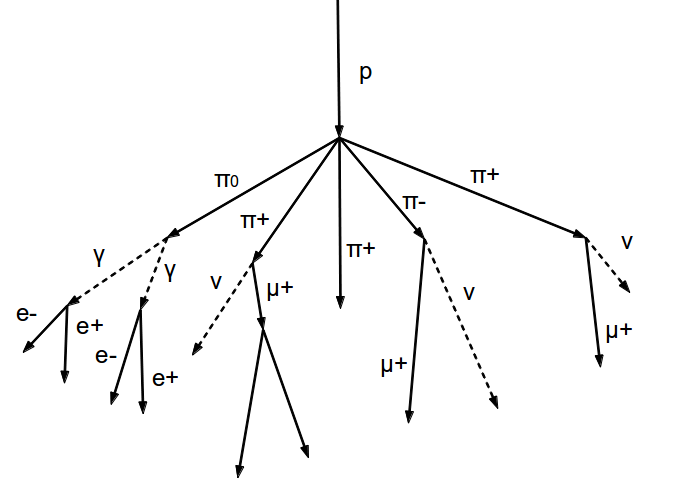
\includegraphics[width=0.45\linewidth]{ProtonDecay.png} \hfill
    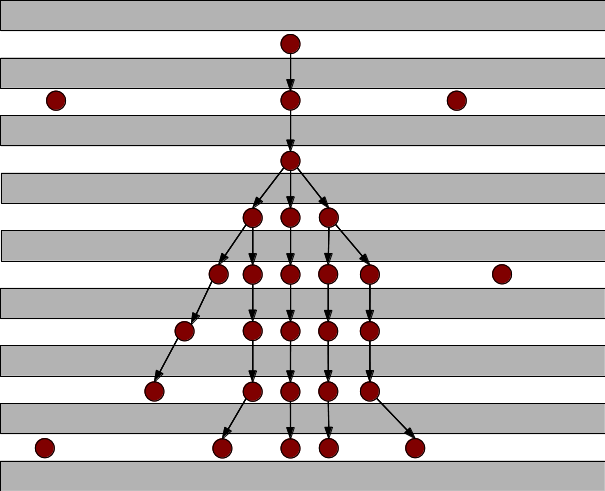
\includegraphics[width=0.45\linewidth]{ArborSchema.png}
  \end{center}
  \caption{\label{ARBOR_STRUCTURE} Left : schematic view of an induced proton shower. Right : schematic view of a reconstructed shower in a calorimeter with calorimeter hits (red)}
\end{figure}

The algorithm we present here is implemented using the PandoraSDK API as a toolkit for generic PFA development \cite{pandora-sdk}. The API is used in a Marlin \cite{marlin-lccd} c++ processor as part of the reconstruction chain in ILCSOFT \cite{ilcsoft}. It produces only a ROOT \cite{root} file containing the variable needed for the analysis described in this document.

Before describing the algorithm contents in detail, few definitions specific to ArborPFA need to be introduced :

\paragraph*{Object} An \textit{object} is a calorimeter hit or a group of contiguous calorimeter hits within a layer that serves as vertex for the ArborPFA algorithm. This was introduced for two reasons i) to provide a generalization of connections between \textit{objects} without making any assumptions of what is contained in an \textit{object}, ii) to overcome the track multiplicity\footnote{More than one pad could be fired when a particle crosses the gas gap.} in gaseous based calorimeters such as SDHCAL \cite{sdhcal-paper}.

\paragraph*{Flow direction} The flow direction is of two kinds : forward direction which is from upstream to downstream of the beam direction and backward direction for the opposite.

\paragraph*{Connector} A connector is a link between two \textit{objects}. It has a weight and a direction.

\paragraph*{Connector depth} The connector depth is defined as the number of intermediary connectors linking two different objects.

\paragraph*{Tree} A tree is a set of \textit{objects} connected in a tree topology which means that for each object there is only one backward connector. An \textit{object} without backward connector is called a seed and an \textit{object} without a forward connector is called a leaf.

\paragraph*{Cluster} A cluster is a set of trees.

\paragraph*{Particle flow object (PFO)} A particle flow object is a set of clusters and tracks \footnote{By track we mean a reconstructed track in tracking detector like a TPC} which corresponds to a reconstructed particle.

~\newline 
Note that in the following algorithm descriptions, some parameters are labelled by a name or a symbol and their values are given in Appendix \ref{ARBOR_ALGORITHM_PARAMETERS}.

\subsection{Pre-clustering phase} 
%%%%%%%%%%%%%%%%%%%%%%%%%%%%%%%%%%%%%%%%%%%

~~~~~~~Before building trees, we need to create objects to connect with each others.

%%% OBJECT CREATION %%%
\begin{wrapfigure}{r}{0.4\textwidth}
  \vspace{-20pt}
  \begin{center}
    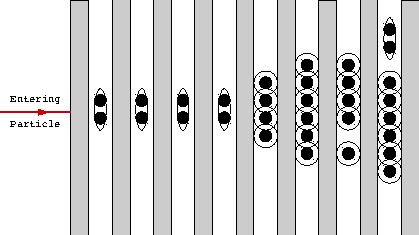
\includegraphics[width=\linewidth]{ObjectCreationAfter.pdf}
  \end{center}
  \vspace{-10pt}
  \caption{\label{ARBOR_OBJECT_CREATION} Schematic view of the object creation output. Small groups of contiguous calorimeter hits are grouped together (encircled).}
  \vspace{-20pt}
\end{wrapfigure}

\paragraph*{Object creation} When a particle goes through the detector, few pads can be fired in a single layer and leads to a multiplicity greater than 1. To overcome the problem, intra-layer group of hits are assembled using the nearest neighbour clustering algorithm. For each group of hits, if its size is greater than 4, the group is split up and each these hits becomes an object. This happens generally in the main part of a shower. Otherwise, an object is created and thus contains from 1 up to 4 calorimeter hits. This is the case for a mip or an isolated group of hits. Figure \ref{ARBOR_OBJECT_CREATION} shows the output of this algorithm with encircled hits forming objects.

%%% MIP TAGGING %%%
\paragraph*{Track segment candidate tagging}
In order to retrieve correctly the primary track in the calorimeter, track segment candidates \textit{objects} are identified and tagged for a future treatment.
For each object, we count the number of neighbouring objects within the same layer at a maximum distance of $\Delta_{mip}$. If this number doesn't exceed N$_{obj,cut}$ it is tagged as a track segment candidate object.

\subsection{The main clustering phase - Connectors and trees}
%%%%%%%%%%%%%%%%%%%%%%%%%%%%%%%%%%%%%%%%%%%

~~~~~~~The main clustering algorithm consists in an iterative procedure using dedicated algorithms in order to create and remove connectors (connector loop). At the end of this step, all the objects are arranged in a tree structure which means that each object has 0 or 1 connector in the backward direction and 0 or many in the forward one.

\begin{figure}[!h]
  \begin{minipage}{0.49\linewidth}
    \begin{center}
      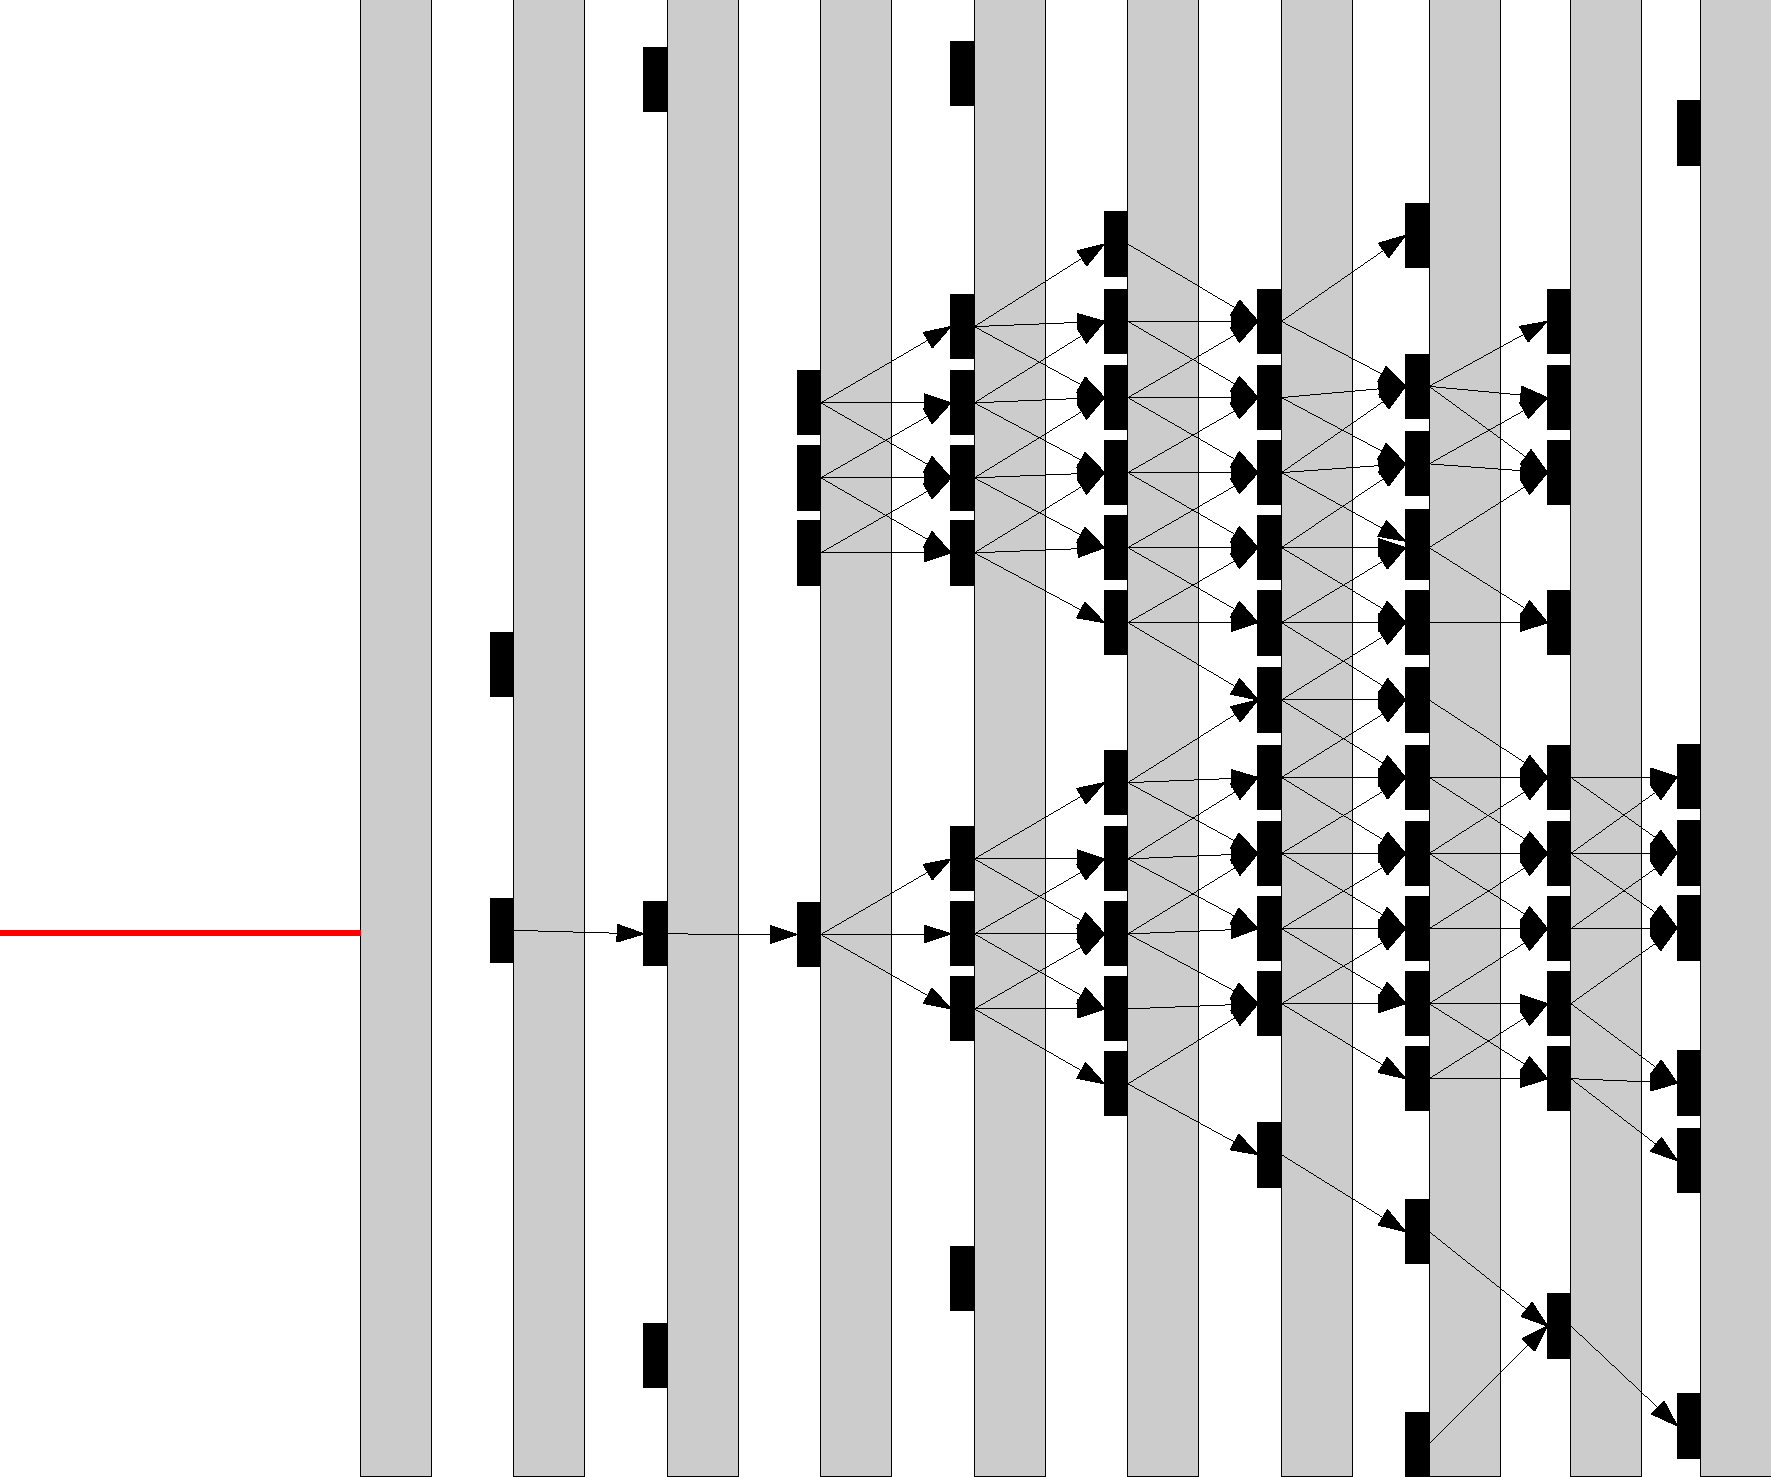
\includegraphics[width=0.9\linewidth]{ConnectorSeeding1.pdf}
    \end{center}
  \end{minipage}
  \begin{minipage}{0.49\linewidth}
    \begin{center}
      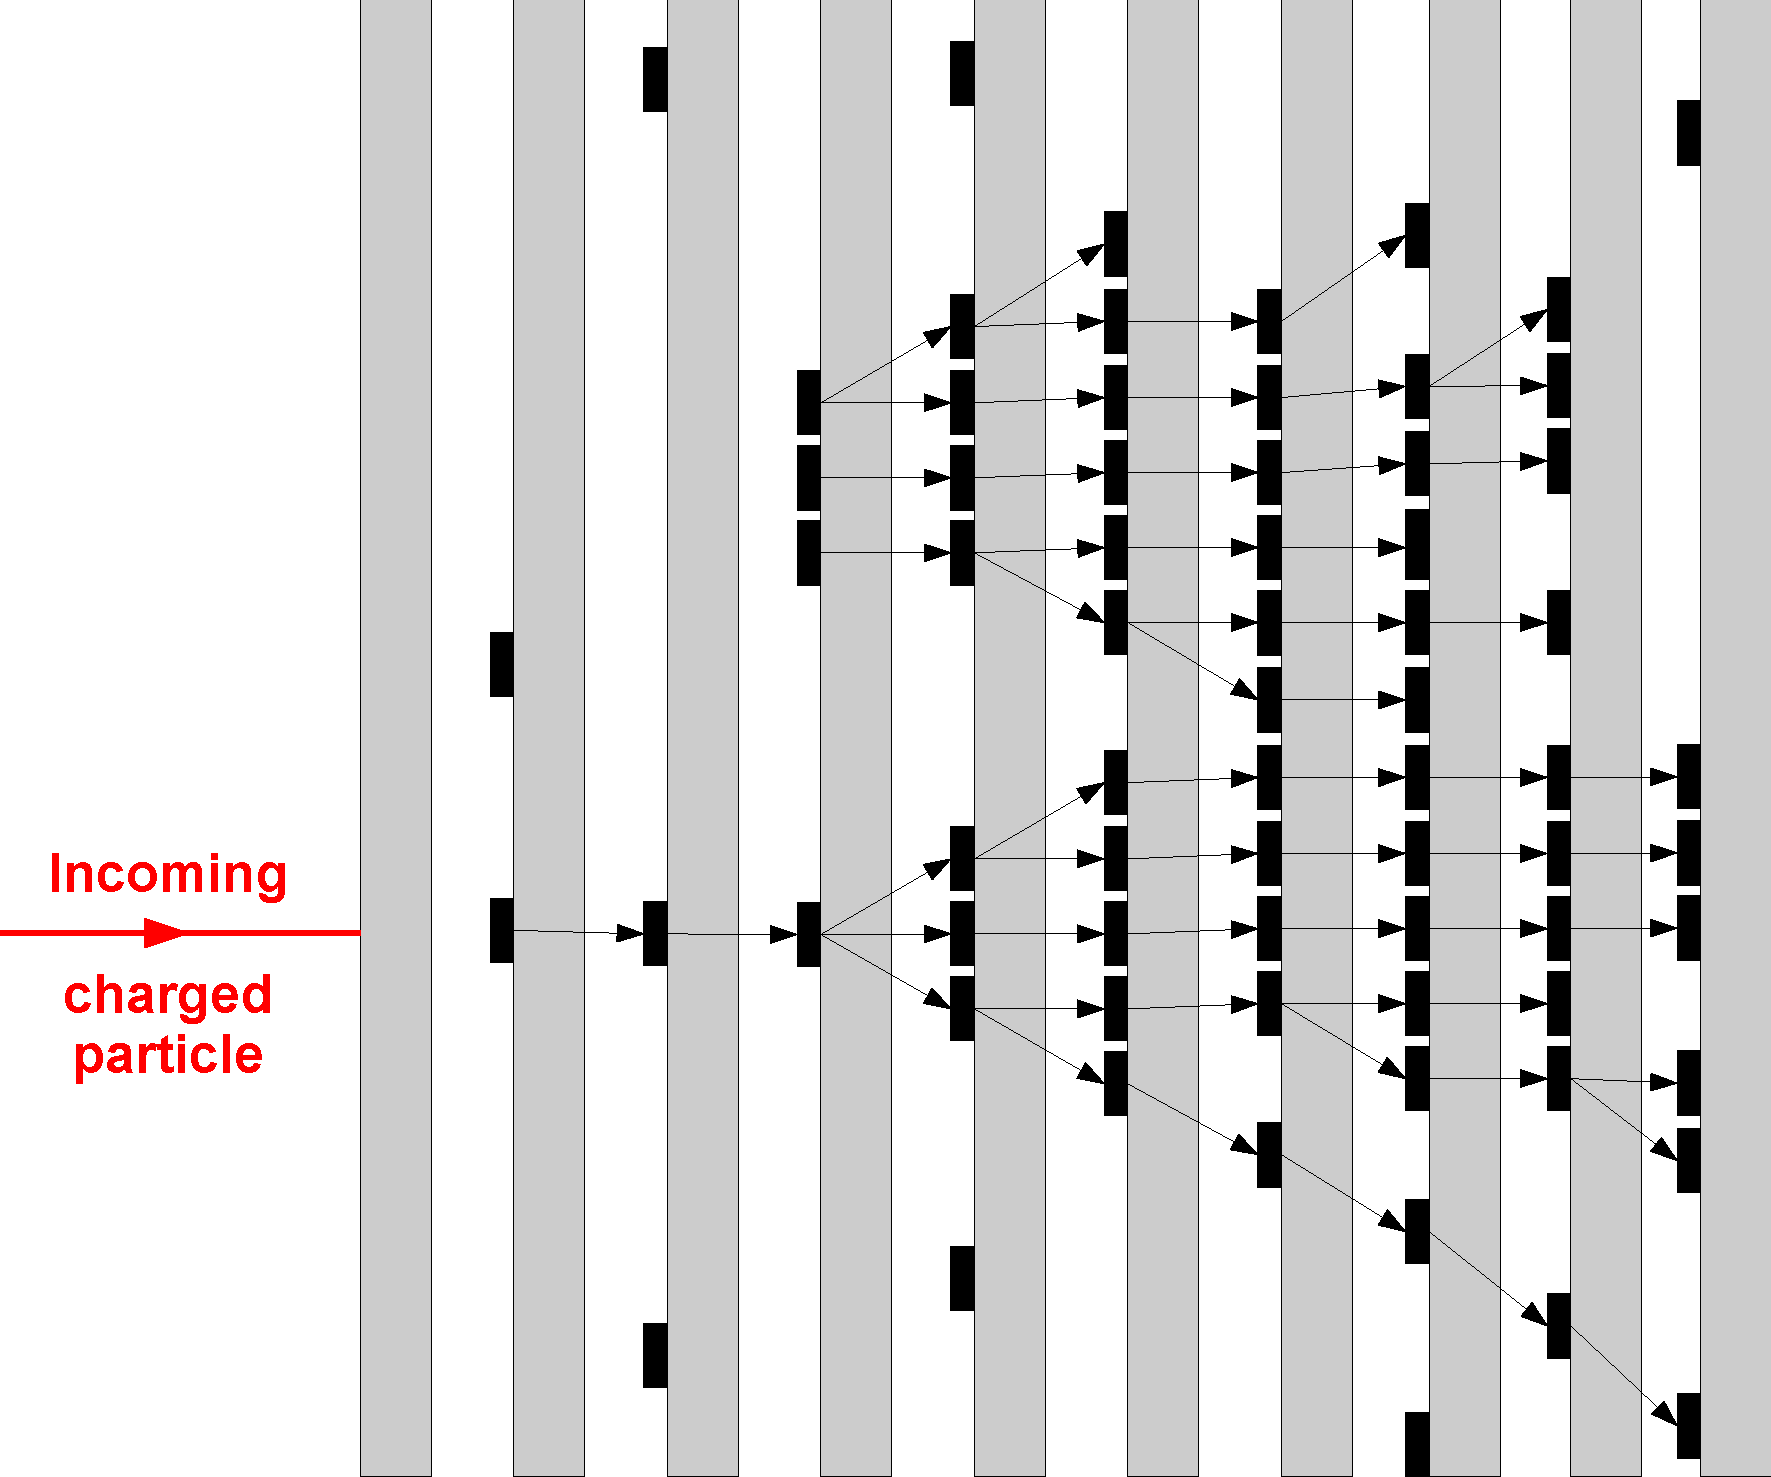
\includegraphics[width=0.9\linewidth]{ConnectorCleaning1.pdf}
    \end{center}
  \end{minipage}
  \caption{\label{ARBOR_CONNECTOR_SEEDING_1} \label{ARBOR_CONNECTOR_CLEANING_1} Schematic view of a neutral and a charged pion showers after the first connector seeding algorithm (left) and cleaning algorithm (right)}
\end{figure}

In the current implementation, the connector loop contains the following algorithms :

\paragraph*{Primary track connection} This algorithm aims to create connections between objects belonging to the primary track of charged particles in the calorimeter. It consists mainly in creating a sub-list of objects that are candidates for the primary tracks by using the objects tagged as track segment candidates and the tracks extrapolation on the calorimeter front face. Once this list is built, the "\textit{connector seeding 1}" algorithm and the "\textit{connector cleaning 1}" algorithm are run on the sub list only. 

\paragraph*{Connector seeding 1} In this sub-part, we start by creating connections in the neighbourhood of each object. For each object, we look for other objects in the N$_{layers}$ next layers with a maximum distance $\Delta_{max}$ and we create a connection between them. Figure \ref{ARBOR_CONNECTOR_SEEDING_1} illustrates the output of this algorithm in one case.

\paragraph*{Connector cleaning 1} Once connectors are seeded, we need to build a tree structure by keeping only one connector in the backward direction for each object. We define the reference direction of an object as :

\begin{equation}
  \vec{C}_{ref} = w_{bck} . \sum_\sigma \sum_b \vec{c}_{b,\sigma} - w_{fwd} . \sum_\delta \sum_f \vec{c}_{f,\delta}
\end{equation}

where :

\begin{itemize}
  \item $w_{bck}$ ($w_{fwd}$) is the global weight assigned to backward (forward) connectors
  \item $\vec{c}_{b,\sigma}$ ($\vec{c}_{f,\delta}$) is the direction of a backward (forward) connector at the connector depth $\sigma$ ($\delta$) from the considered object
\end{itemize}

The depth parameter $\sigma$ has been fixed to 1 in all algorithms. The reference direction is a vector that goes in the backward direction and indicates the most probable direction for a unique backward connection. Then we need to assign which backward connector should be kept for the tree building. Thus, for each backward connector of an object, we define the $\kappa$ order parameter as :

\begin{equation}
  \kappa~=~\Big(\frac{\theta}{\pi}\Big)^{p_{\theta}} . ~\Big(\frac{\Delta}{\Delta_{max}}\Big)^{p_{\Delta}} 
\end{equation}

where :

\begin{itemize}
  \item $\theta$ is the angle between a backward connector and the reference direction of the considered object,
  \item $\Delta$ is the distance between a pointed backward object and the considered object,
  \item $p_{\theta}$ (resp. $p_{\Delta}$) is a power parameter for the normalized angle (resp. the normalized distance)
\end{itemize}

The $\kappa$ parameter quantifies the alignment with the reference direction within the range [0,1]. Smaller is this parameter, higher the alignment will be. Thus, the power parameters $p_{\theta}$ and $p_{\Delta}$ are to be tuned depending on which variable we want to emphasize.

The chosen backward connector for the tree building will be the one with the smallest $\kappa$ parameter; all the others are removed from the list. The removal of connectors is done at the end of the algorithm such that all connectors contribute to the evaluation of the reference direction.

\begin{figure}[!h]
  \begin{minipage}{0.4\linewidth}
    \begin{center}
      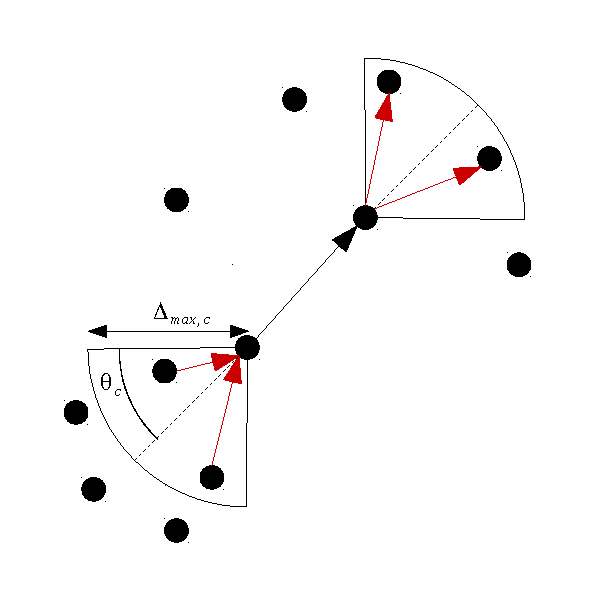
\includegraphics[width=0.8\linewidth]{ConnectorAlignment.pdf}
    \end{center}
  \end{minipage}
  \begin{minipage}{0.58\linewidth}
    \begin{center}
      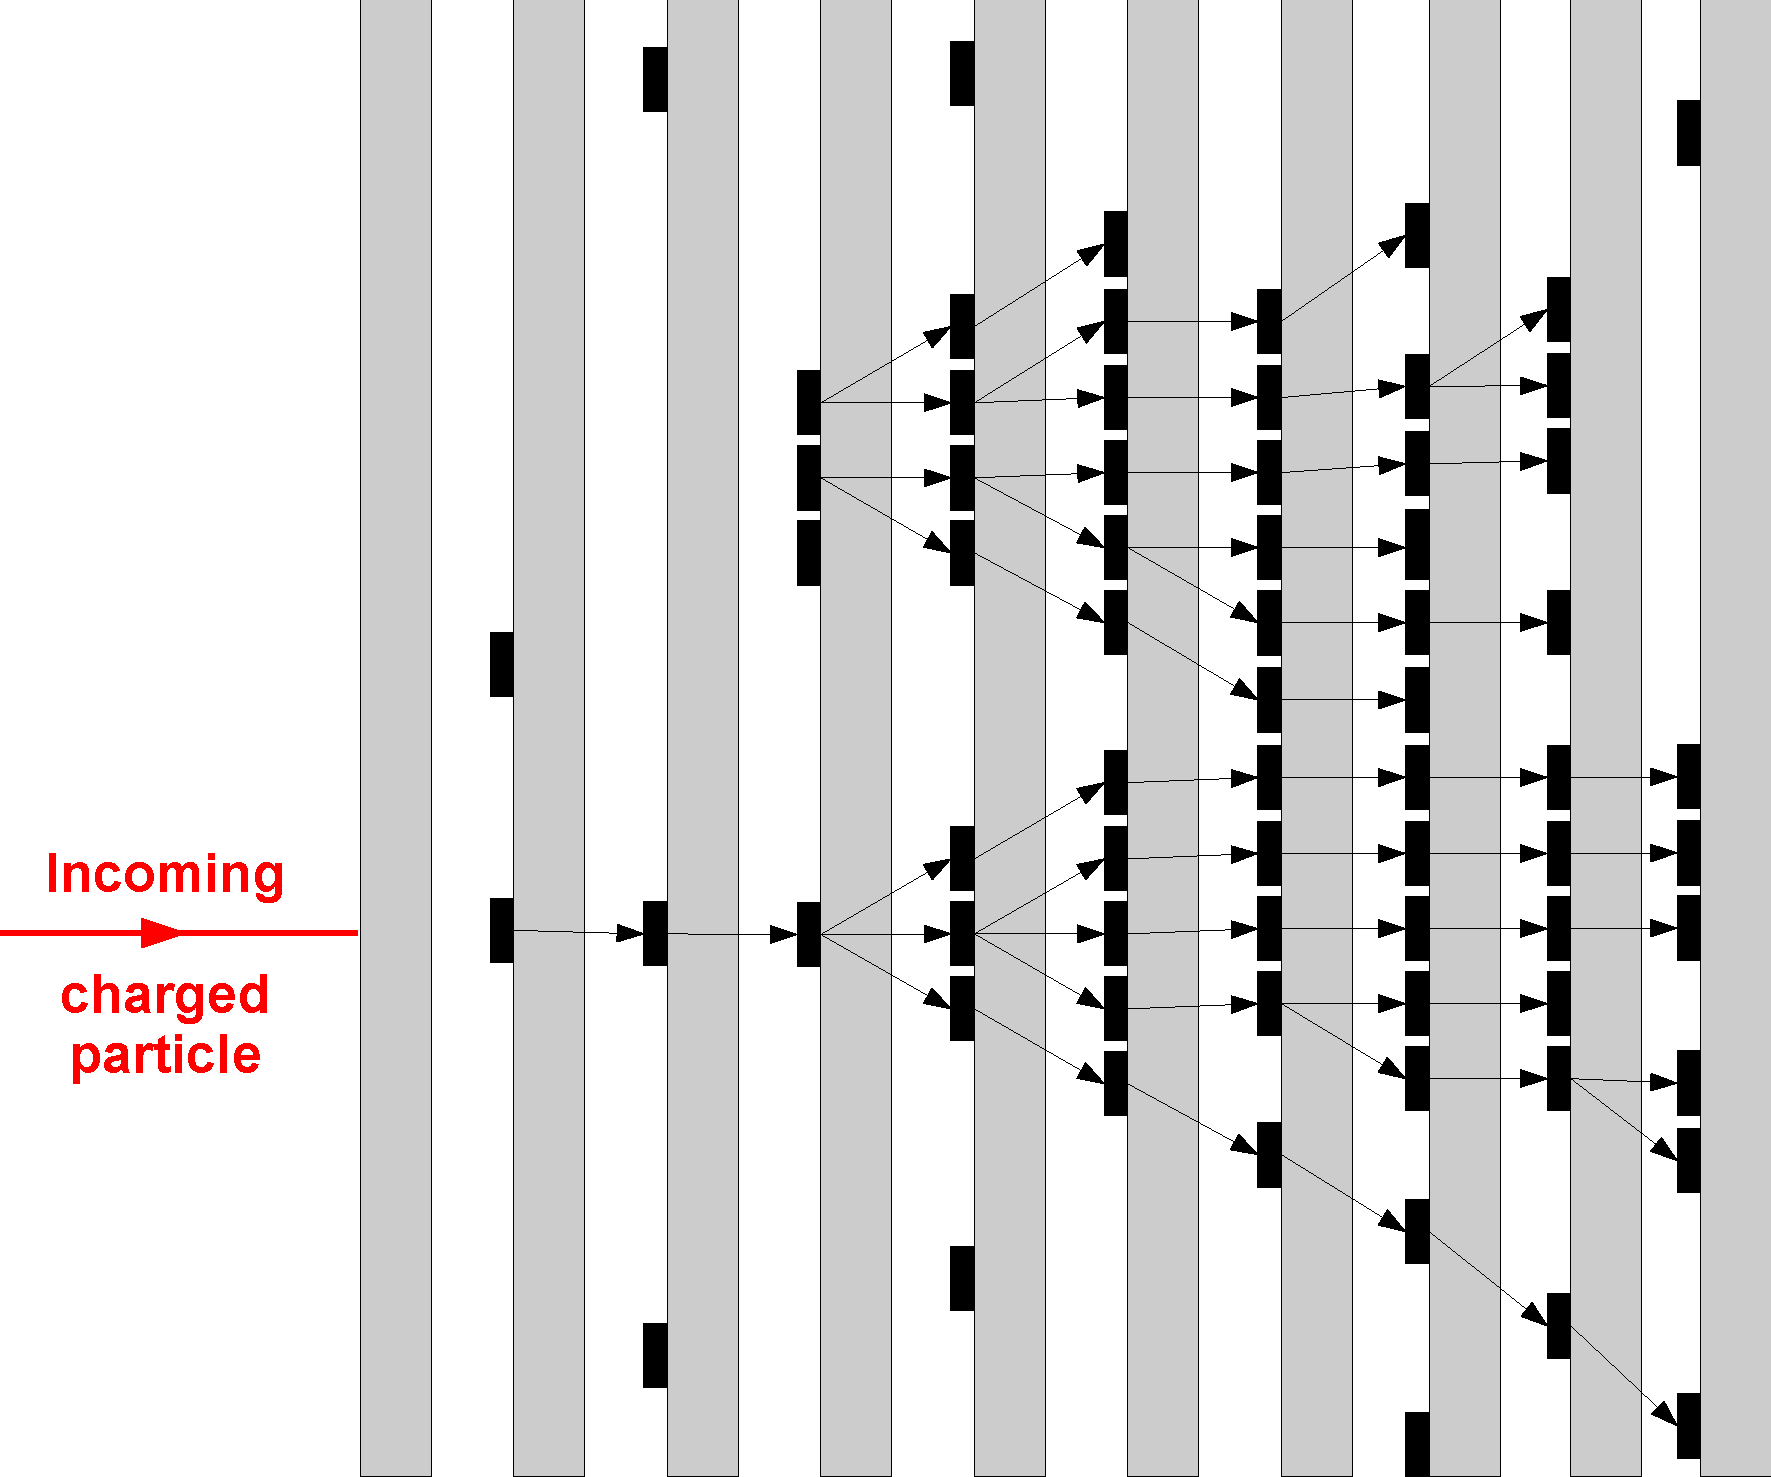
\includegraphics[width=0.8\linewidth]{ConnectorCleaning2.pdf}
    \end{center}
  \end{minipage}
  \caption{\label{ARBOR_CONNECTOR_ALIGNEMENT} \label{ARBOR_CONNECTOR_CLEANING_2} Left : Schematic view of the connector alignment procedure. In black, a considered connector and in red possible new connectors in backward and forward directions. Right : a neutral and a charged pion showers after the second connector cleaning algorithm}
\end{figure}

\paragraph*{Connector seeding 2} This second step of connector seeding starts from the tree structure obtained after the first connector cleaning algorithm. The goal of this second step is to create an alignment of connectors within the shower. For each connector, more forward connectors are created from the forward object of this connector by looking in a cone of half-angle $\theta_c$ and a maximum distance of $\Delta_{max,c}$. In the same way, more backward connectors are created from the backward object of this connector. A schematic view of this step is shown on figure \ref{ARBOR_CONNECTOR_ALIGNEMENT}.

\paragraph*{Connector cleaning 2} Here, we need again to clean-up the backward connector list to end up with only one connector. This last algorithm is similar to the first connector cleaning except that the cleaning is done layer per layer starting from the downstream layers with a depth parameter $\delta$ strictly higher than one. For a given connector, this accentuates the alignment with the forward ones. We end up then with a tree structure again.

\paragraph*{Tree building} This step is straight-forward. Seed objects are identified and trees are built by following the forward connected objects recursively. At this step, clusters are built each containing a single tree. The following algorithms will associate some of the trees with others.

%%%%%%%%% ASSOCIATION ALGORITHMS %%%%%%%%%%%
\subsection{Association algorithms}

\paragraph*{Energy driven track cluster association} The track to cluster association is performed using two different information, the energy/momentum of the cluster/track and the cluster topology. We first look at the track projection at the calorimeter front face. Two different cases may happen :

\begin{itemize}
  \item the particle has interacted before the calorimeter or in the first layer. In this case, many seed objects are found in the N$_{layer}$ first layers at a maximum distance of $\Delta_{{track-cluster}_1}$ of the track projection. Seed objects are then sorted by their distance to the track projection. The clusters associated to their seeds are then associated to the track progressively starting from the closest one until the difference between the track momentum and the total cluster energy is minimized. The associated clusters of a track are then merged since they belong to the same cluster structure.
  \item the particle produced a track segment at least in the N$_{layer}$ first layers and a seed objects are found within a distance $\Delta_{(track-cluster)_1}$ to the track projection. Since only a cluster starting with a track segment has to be associated, an additional distance cut $\Delta_{(track-cluster)_2}$ between seed objects and the track projection is applied. This decreases the confusion for a small separation distance between close by particles. The same track-to-cluster association and cluster merging is then performed as above.
\end{itemize}

\begin{minipage}{0.58\linewidth}
  \vspace{-2ex}
  \begin{center}
    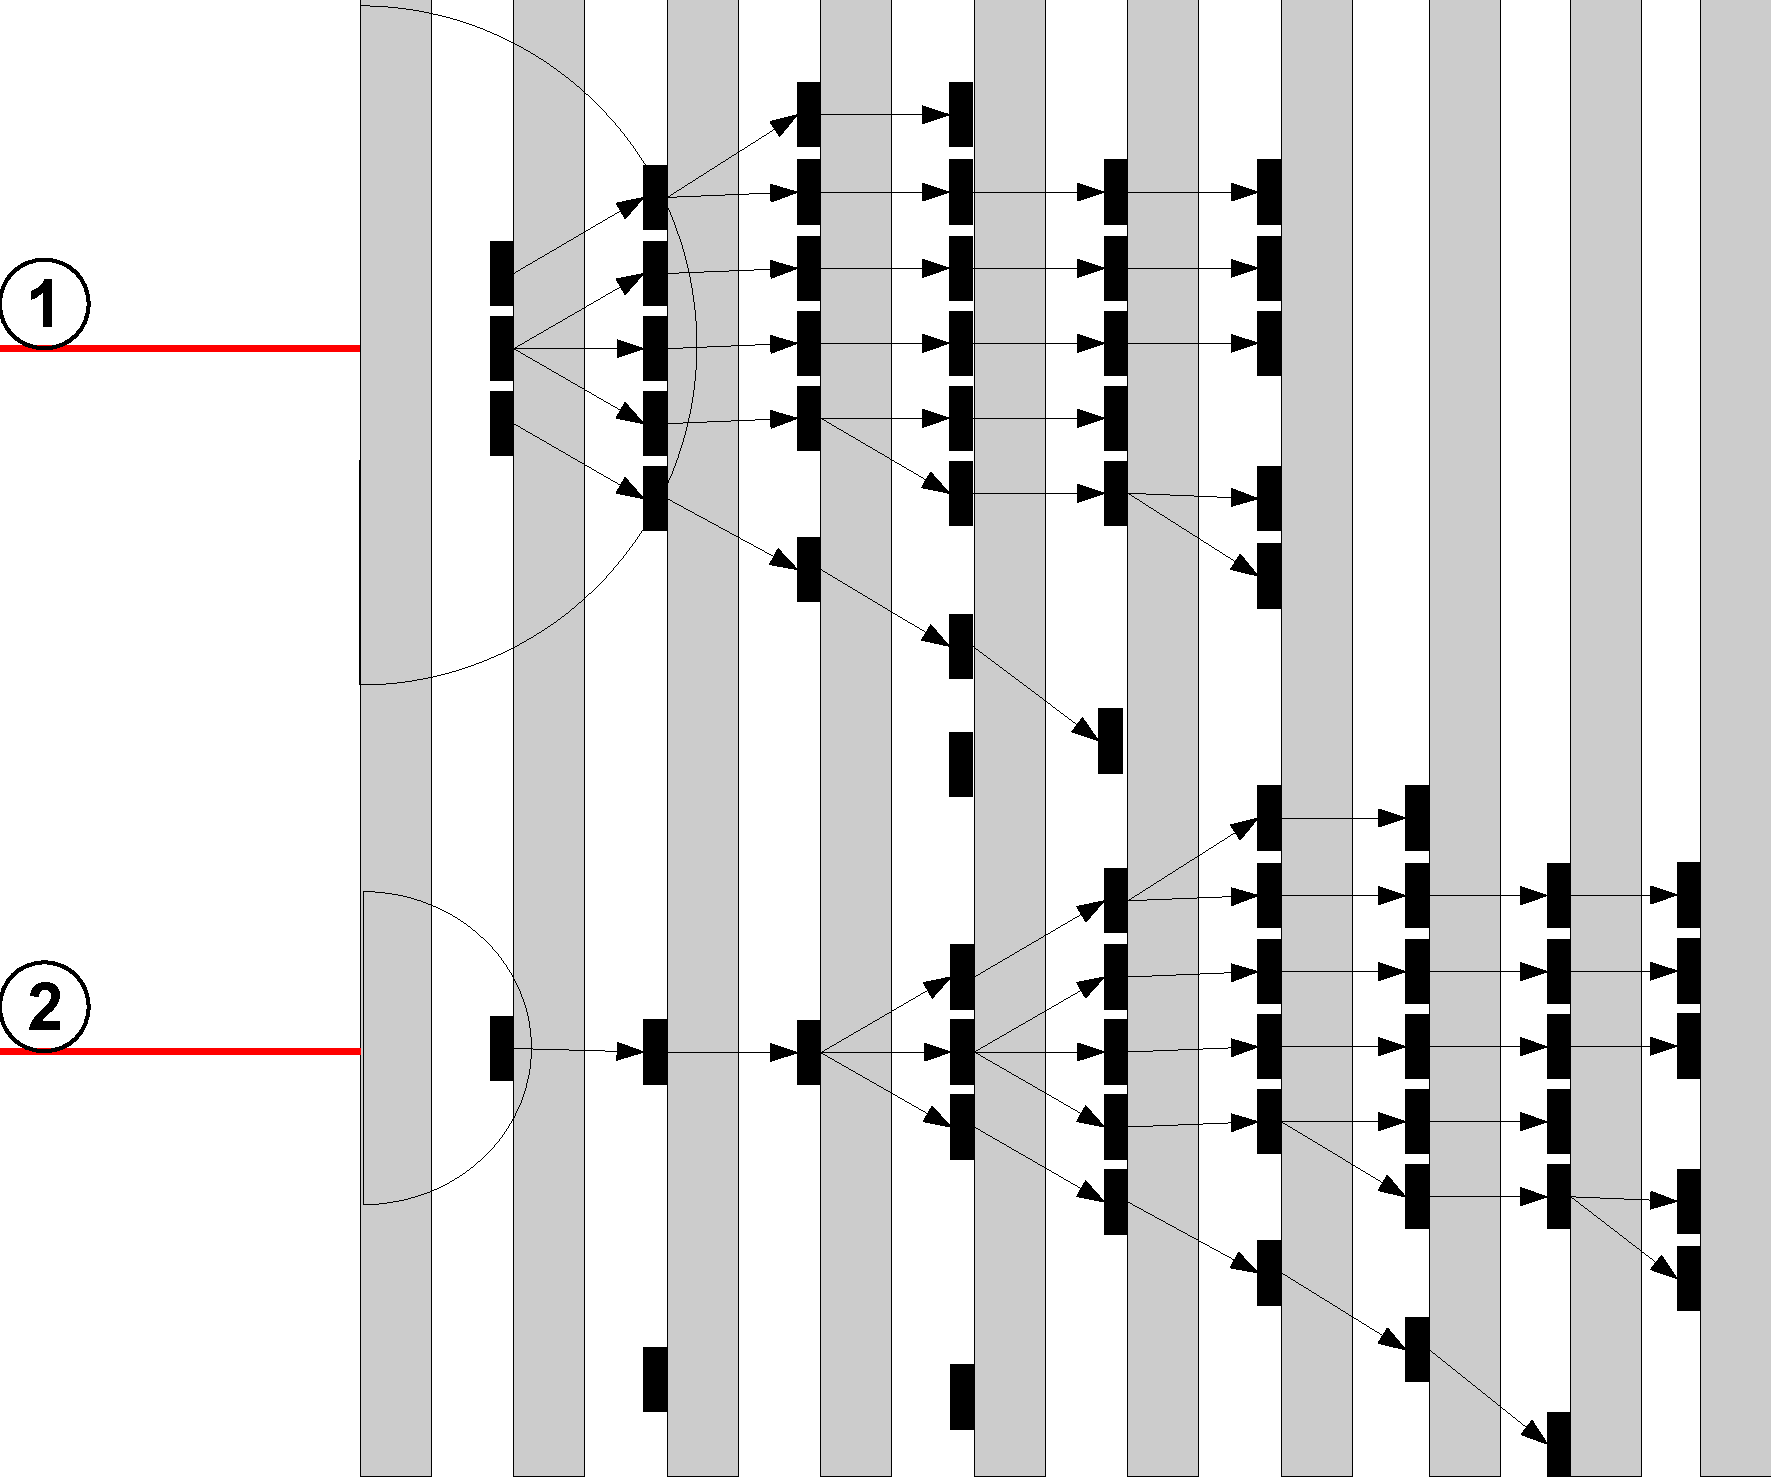
\includegraphics[width=0.7\linewidth]{EnergyDrivenTrackClusterAssociation.pdf}
    \captionof{figure}{\label{ARBOR_ENERGY_DRIVEN_TRACK_CLUSTER_ASSOCIATION} Schematic view of the energy driven track cluster algorithm.}
  \end{center}
\end{minipage}
\begin{minipage}{0.4\linewidth}
  \vspace{-2ex}
  \begin{center}
    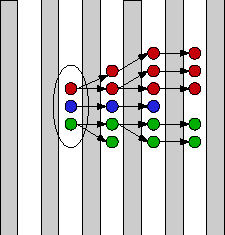
\includegraphics[width=0.8\linewidth]{NeutralTreeMerging.pdf}
    \captionof{figure}{\label{ARBOR_NEUTRAL_TREE_MERGING} Schematic view of the neutral tree merging algorithm.}
  \end{center}
\end{minipage}
\newline

Figure \ref{ARBOR_ENERGY_DRIVEN_TRACK_CLUSTER_ASSOCIATION} shows a schematic view of the two different scenarios. The first one corresponds to the case where an early interaction is found and the second one where a primary track segment of a cluster is found.

\paragraph*{Neutral tree merging} This algorithm is designed for neutral particle interactions for which the first interacting layer contains few seeds. Figure \ref{ARBOR_NEUTRAL_TREE_MERGING} shows a configuration where many trees have been built (with three colours) for one neutral particle interaction. We can see that the seeds in the first interacting layer belongs to the same cluster. We group all the tree seeds within the same layer and at maximum distance of $\Delta_{seed}$. Then all of these trees are merged in the cluster.

\paragraph*{Pointing cluster association} This step aims at associating neutral fragments to other fragments which may be charged or neutral parent clusters. We start by identifying the clusters that have at least N$_{objects}$ objects in at least N$_{layer}$ contiguous layers. The selected cluster could be either a parent or a daughter cluster. Then we proceed as follows :

\begin{enumerate}
  \item A linear 3D straight line fit is performed over the position of all the hits of each cluster. This defines the direction of each cluster.
  \item The clusters are sorted by their most downstream layers (downstream hit in the cluster) l$_{inner}$.
  \item Starting from the most downstream cluster \textit{i}, we look for a parent cluster \textit{j} for which l$_{inner,i}$~>~l$_{inner,j}$.
  \item Among these candidate parent clusters, we look for those for which d$_{proj}$ < d$_{proj,cut}$ \& $\theta_{i,j}$ < $\theta_{i,j,cut}$  where :
  \begin{itemize}
    \item d$_{proj}$ is the distance between the candidate daughter cluster direction and the candidate parent cluster barycentre (line-to-point distance)
    \item $\theta_{i,j}$ is the angle between the direction of the two clusters
  \end{itemize}
  and we choose the cluster for which d$_{proj}$ is minimum.  
  \item Among this same list of candidate parent clusters, we look for those satisfying the condition d$_{cross}$ < d$_{cross,cut}$ \& d$_{closest}$ < d$_{closest,cut}$ where :
  \begin{itemize}
    \item d$_{cross}$ is the distance at closest approach (d.c.a) between the two cluster directions
    \item d$_{closest,i,j}$ is the closest distance between an object of the parent cluster and the point where the daughter cluster direction crosses the parent one (distance at closest approach) 
  \end{itemize}
  and we choose the cluster for which d$_{cross}$ is minimum.
  \item We choose the best candidate parent cluster among the two previous methods above. Many cases may happened i) no parent cluster is found, then no parent cluster is assigned to this daughter cluster, ii) one of the two methods has found a parent cluster or the two methods provide the same parent, then we assign it to the daughter cluster, iii) the two methods have found a parent cluster but there are not the same one. In this case the closest candidate parent cluster among the two in terms of barycentre distance is assigned to the daughter cluster.
  \item If no parent cluster has been found for the cluster \textit{i}, stop processing this cluster, else :
  \item If the parent cluster has no associated track, merge the two clusters, else :
  \item We define the variable $\Psi$ as :
  \begin{equation}
    \label{PSI2_ALGORITHM_EQUATION}
    \Psi = \Big| \frac{p-E_{tot}}{f_{res} . \sigma_E . p} \Big|
  \end{equation}
  where :
  \begin{itemize}
    \item p is the track momentum of the parent cluster
    \item E$_{tot}$ is the total energy estimated from the combined hit list of the parent and daughter clusters
    \item $\sigma_E$ is the energy resolution at the track momentum p 
    \item f$_{res}$\footnote{The parameter f$_{res}$ is used to reduce or enlarge the accepted range of the difference p-E$_{tot}$. A higher value of this parameter will accept a merging with a higher difference p-E$_{tot}$.} is an energy resolution factor
  \end{itemize}
  
\begin{figure}[!h]
  \begin{center}
    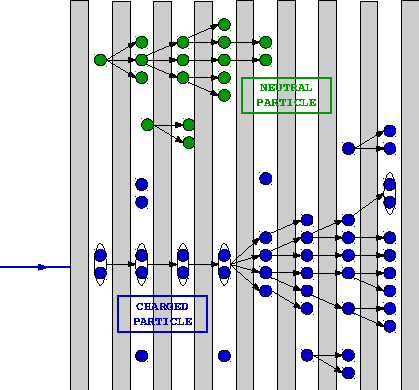
\includegraphics[width=0.4\linewidth]{PfoCreation.pdf}
  \end{center}
  \caption{\label{ARBOR_PFO_CREATION} Schematic view of the final ArborPFA output}
\end{figure}

We check then that the $\Psi^2$ defined for the parent and daughter clusters is less than $\Psi^2_{cut}$ and if the difference between p and E$_{tot}$ after the cluster merging (parent + daughter clusters) decreases. The two clusters are merged if the previous conditions are satisfied.

\end{enumerate}

\paragraph*{Small neutral fragment merging} At this stage, the main part of the shower of each particles has been identified. Only isolated objects and small tree structures that surrounds the showers are not associated. First, these small structures are identified if their size is less than $N_{cut}$ objects. Then for all showers and small structures, the centroid (barycentre) is computed and each small structure is merged in the shower that has the smallest distance between centroids.

\paragraph*{Particle flow object creation} Particle flow objects are built from the produced clusters after all the steps described above (Figure \ref{ARBOR_PFO_CREATION}). Charged PFOs are built from clusters that have an associated track, while other clusters are considered as neutral PFOs.

%%%%%%%%%%%%%%%%%%%%%%%%%%%%%%%%%%%
%%%%%% Single particle study %%%%%%
%%%%%%%%%%%%%%%%%%%%%%%%%%%%%%%%%%%
\newpage
\section{Single particle study}
\label{SINGLE_PARTICLE_STUDY_SECTION}

\subsection{Setup}

\begin{wrapfigure}{r}{0.45\textwidth}
  \vspace{-20pt}
  \begin{center}
    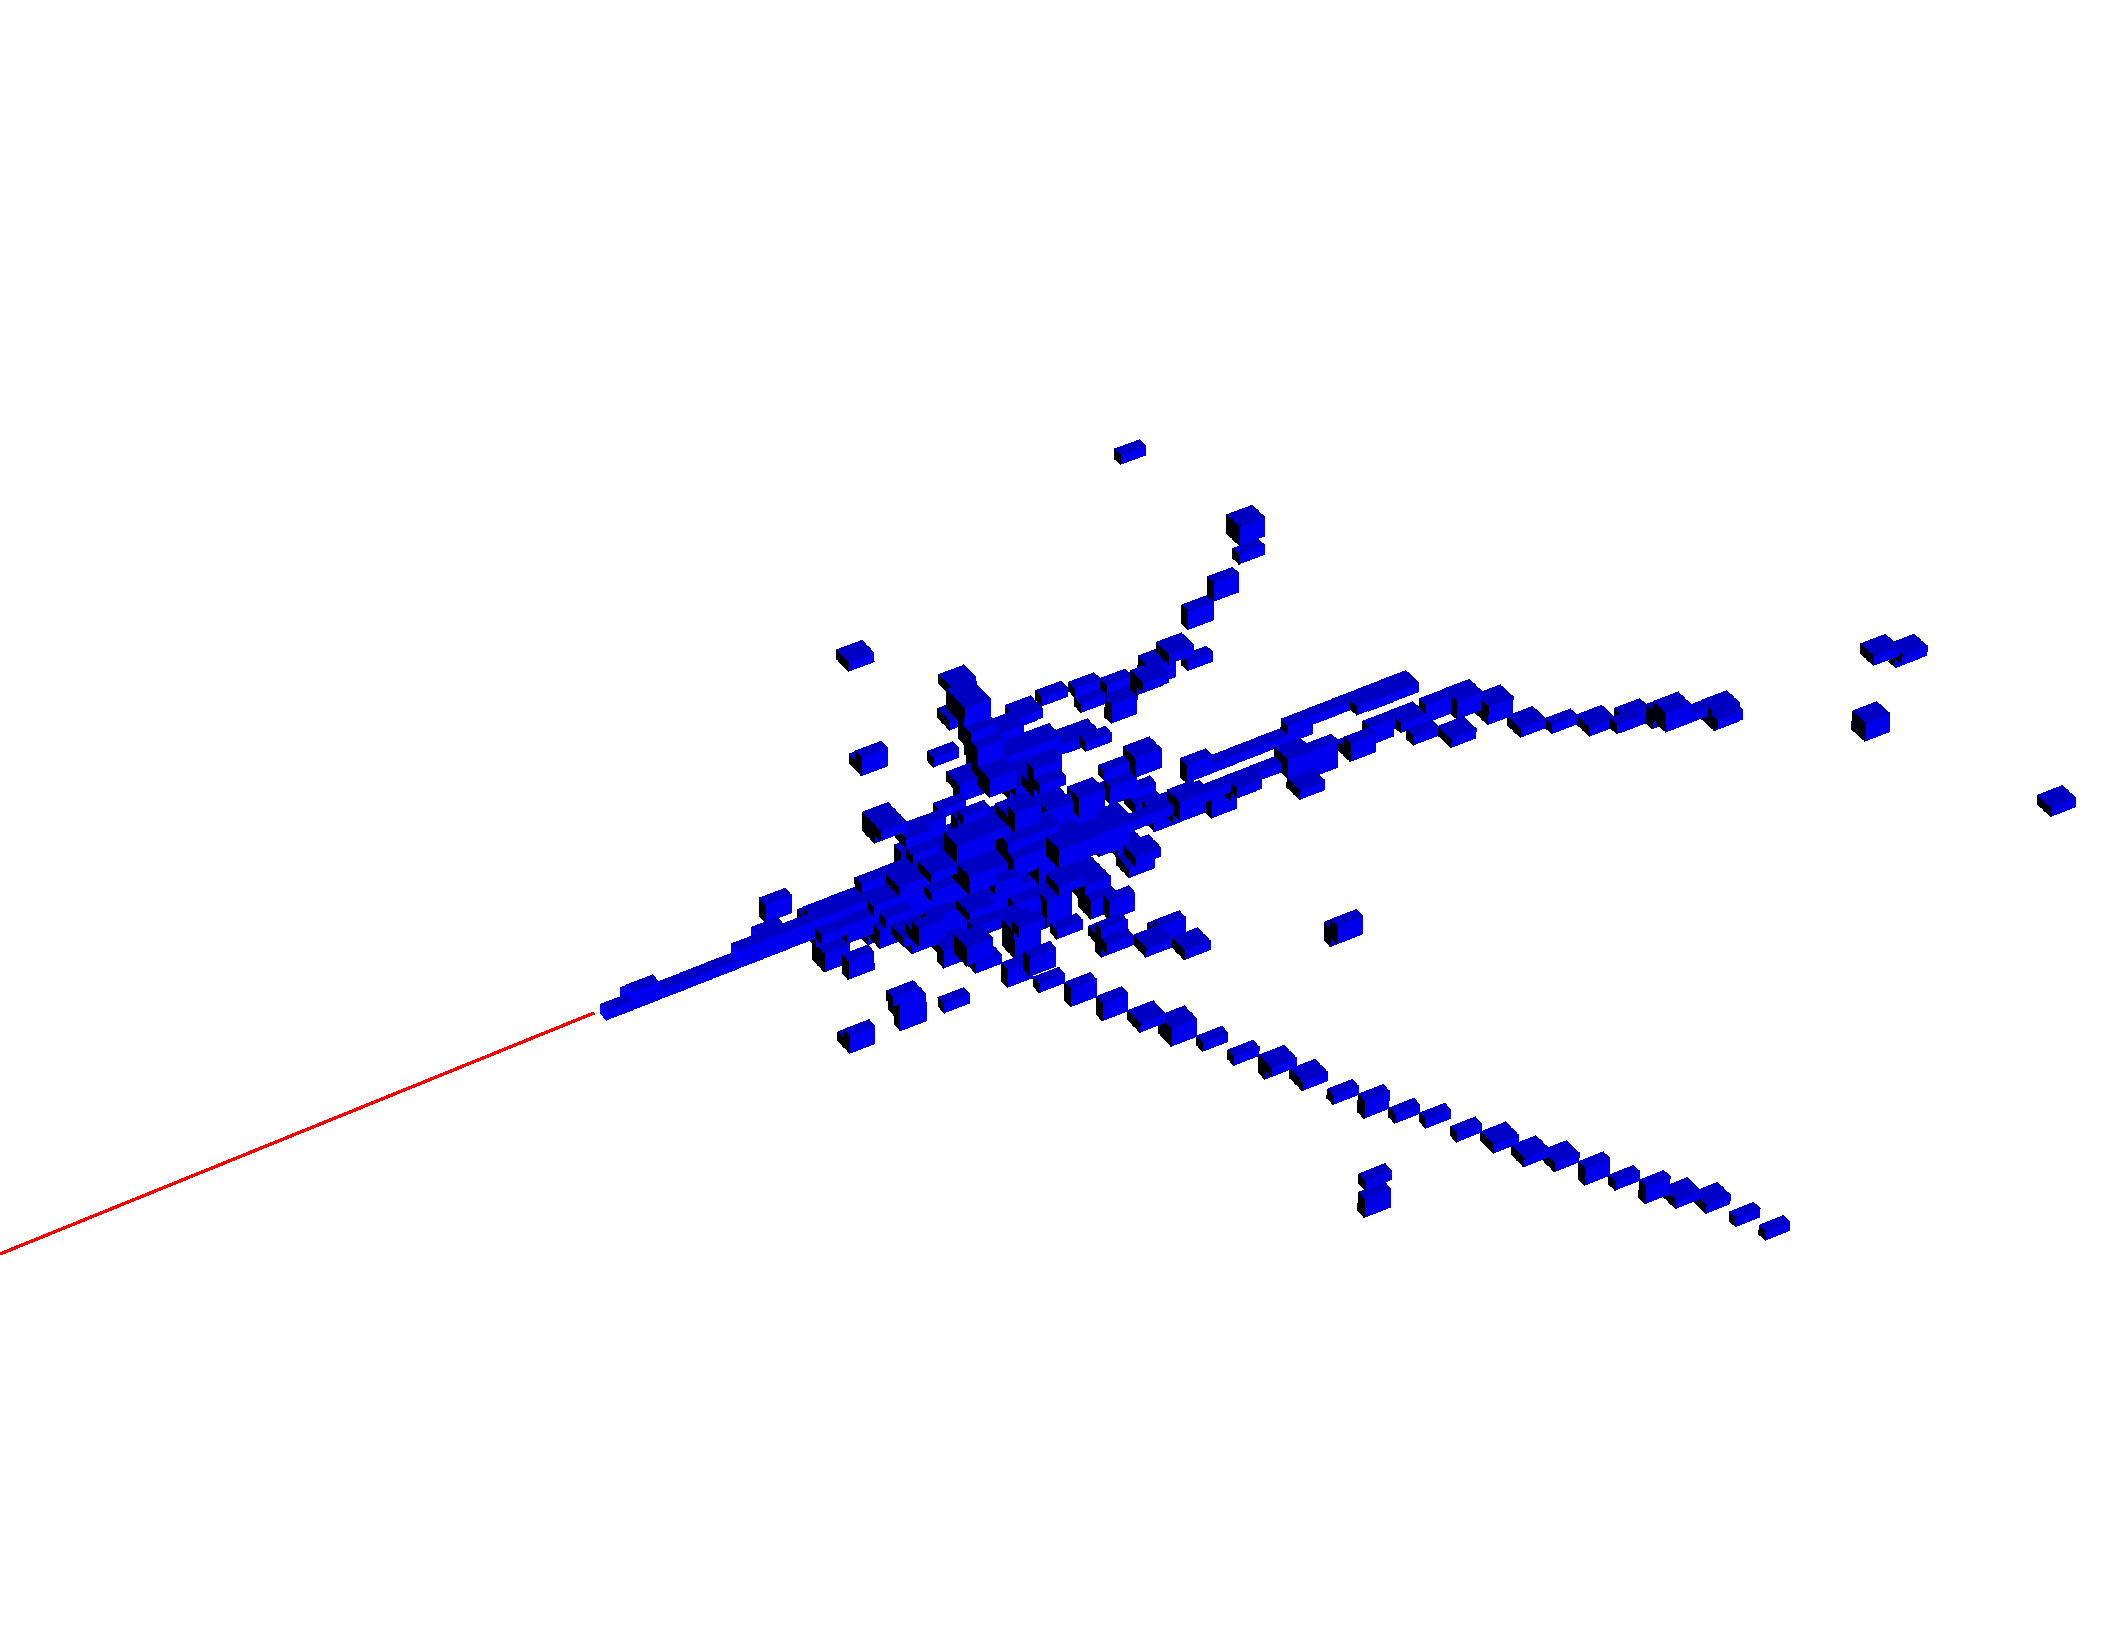
\includegraphics[width=\linewidth]{SingleParticleSetup.pdf}
  \end{center}
  \vspace{-10pt}
  \caption{\label{ARBOR_SINGLE_PARTICLE_SETUP} Event display of a 50 GeV pion shower in the SDHCAL detector as loaded in the reconstruction framework}
\end{wrapfigure}

To study the single particle performance, we use the SDHCAL charged pion data taken at CERN on the H6 line of SPS in 2012. The list of runs for the different energies can be found in Appendix \ref{SDHCAL_RUN_LIST}. In order to select only pions, an event selection is performed as described in \cite{sdhcal-paper}.

To emulate correctly a charged pion for the reconstruction program, a fake-track is created in front of the calorimeter. A global barycentre of the whole hit positions in the transverse plan is calculated. A new barycentre is then calculated using the 4 first layers only and within a region of 8x8 cells around the global barycentre in the x and y direction. This defines the shower entering point in the first layer. From the entering point of the shower, a straight track is created with a momentum which has the beam's one.

The inputs are then loaded in the PandoraSDK toolkit \cite{pandora-sdk} within a single hcal endcap geometry (without the beam pipe and the BeamCal) and processed by the ArborPFA algorithms. An event display after loading the inputs in the framework is shown on figure~\ref{ARBOR_SINGLE_PARTICLE_SETUP}.

\subsection{Single particle analysis}

\begin{figure}[!h]
  \begin{center}
    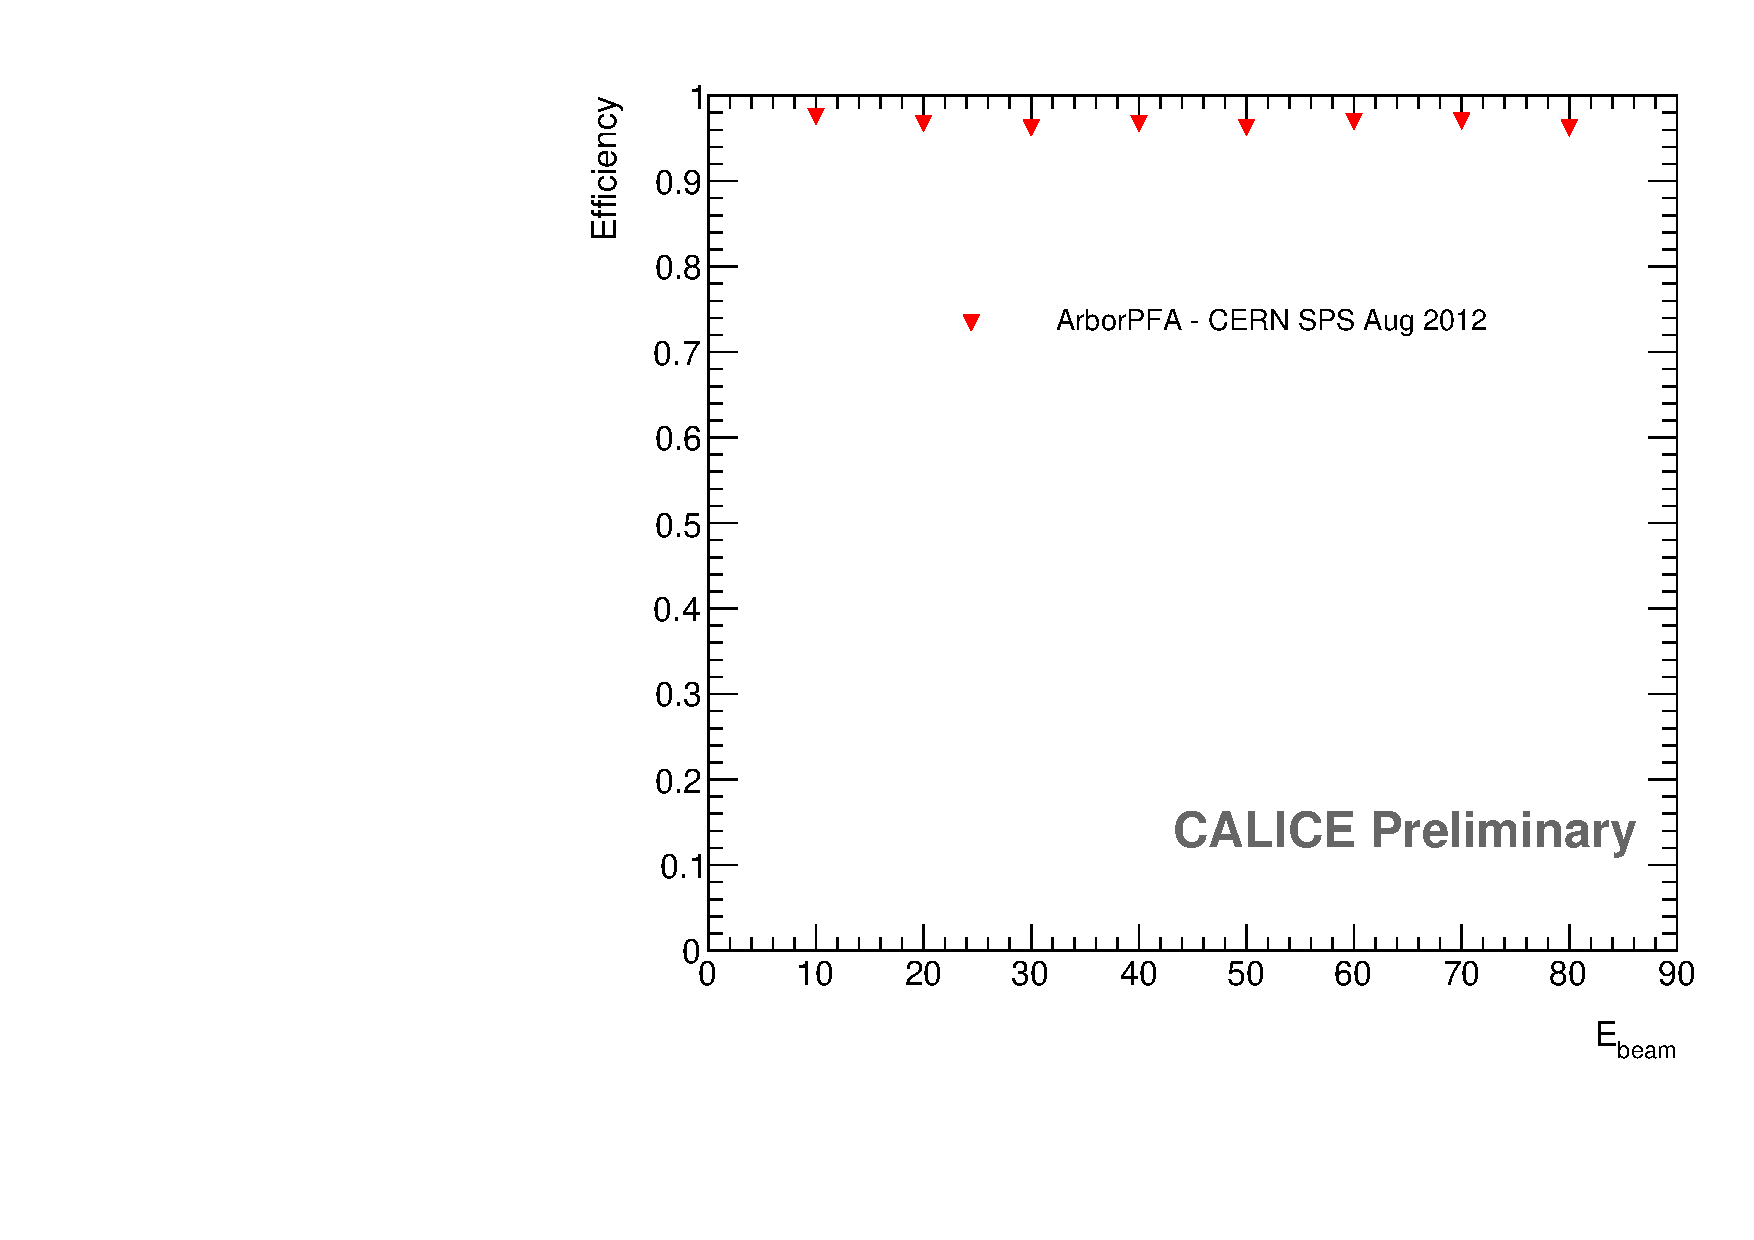
\includegraphics[width=0.48\textwidth]{plots/SingleParticle_Efficiency.pdf}
    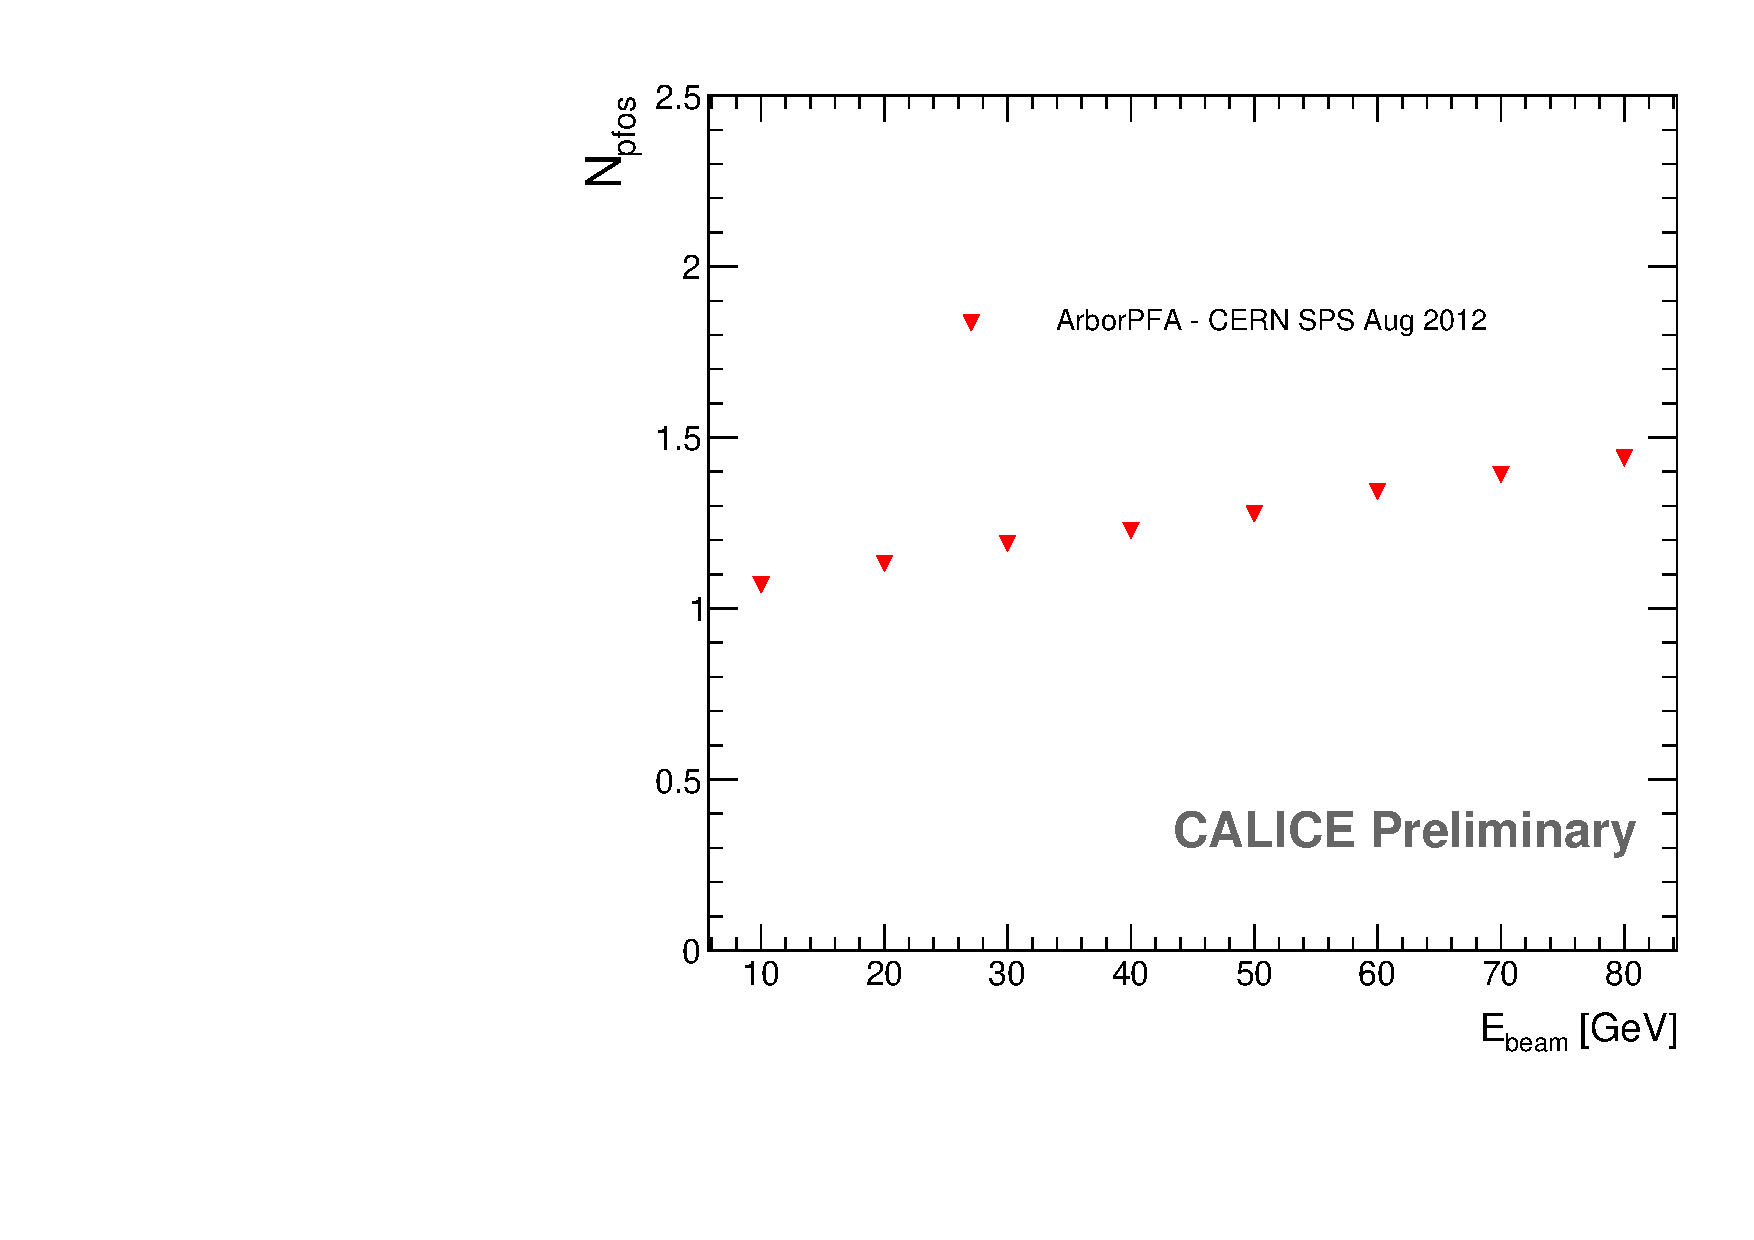
\includegraphics[width=0.48\textwidth]{plots/SingleParticle_NPfos.pdf} \\
  \end{center}
  \caption{\label{ARBOR_SINGLE_PARTICLE_EFFICIENCY_AND_NPFOS} Efficiency of the number of recovered hits (left) and the mean number of reconstructed particles (right) after ArborPFA reconstruction on single pion shower events with the SDHCAL prototype}
\end{figure}

We define the efficiency of the single particle reconstruction $\epsilon_s$ as the number of hits recovered by the ArborPFA program and correctly attached to track in front of the calorimeter. Figure \ref{ARBOR_SINGLE_PARTICLE_EFFICIENCY_AND_NPFOS} shows the mean efficiency of the single particle reconstruction (left) and the mean number of reconstructed particles (right) as a function of the beam energy after applying the ArborPFA. It shows a constant efficiency with more than 95\% over the whole beam energy range. But since the number of hits increases with the energy, the number of missed hits in the reconstructed charged particle increases as well. Consequently, the number of reconstructed particles shows an increase which is directly due to the shower splitting. This number grows up to 1.45 particles at 80 GeV but has finally a small impact on the reconstructed energy and energy resolution because the small additional clusters represent a small amount of energy. Indeed, figure \ref{ARBOR_SINGLE_PARTICLE_EREC_AND_ERESOL} shows the reconstructed energy and energy resolution of a single charged pion before and after running the ArborPFA program. 

\begin{figure}[!h]
  \begin{center}
    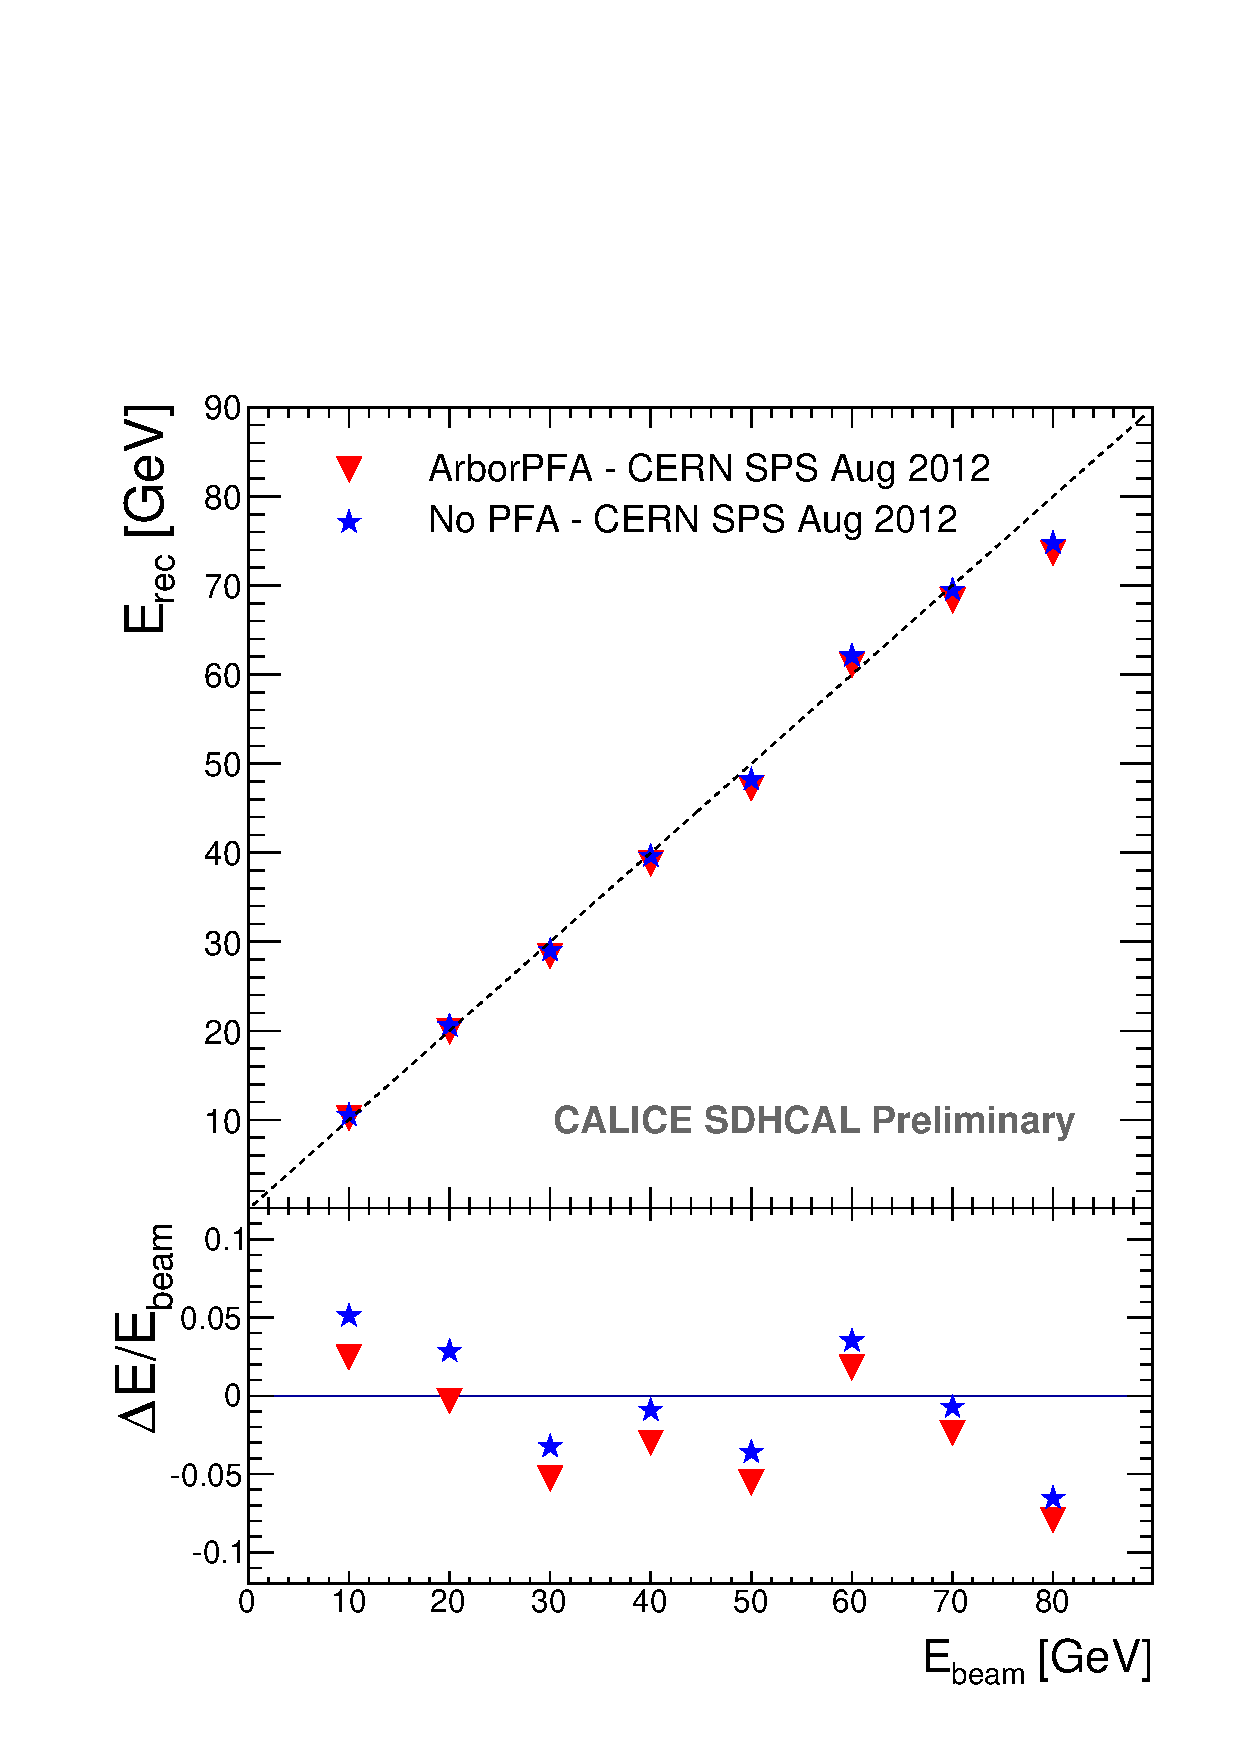
\includegraphics[width=0.48\textwidth]{plots/SingleParticle_ERec.pdf}
    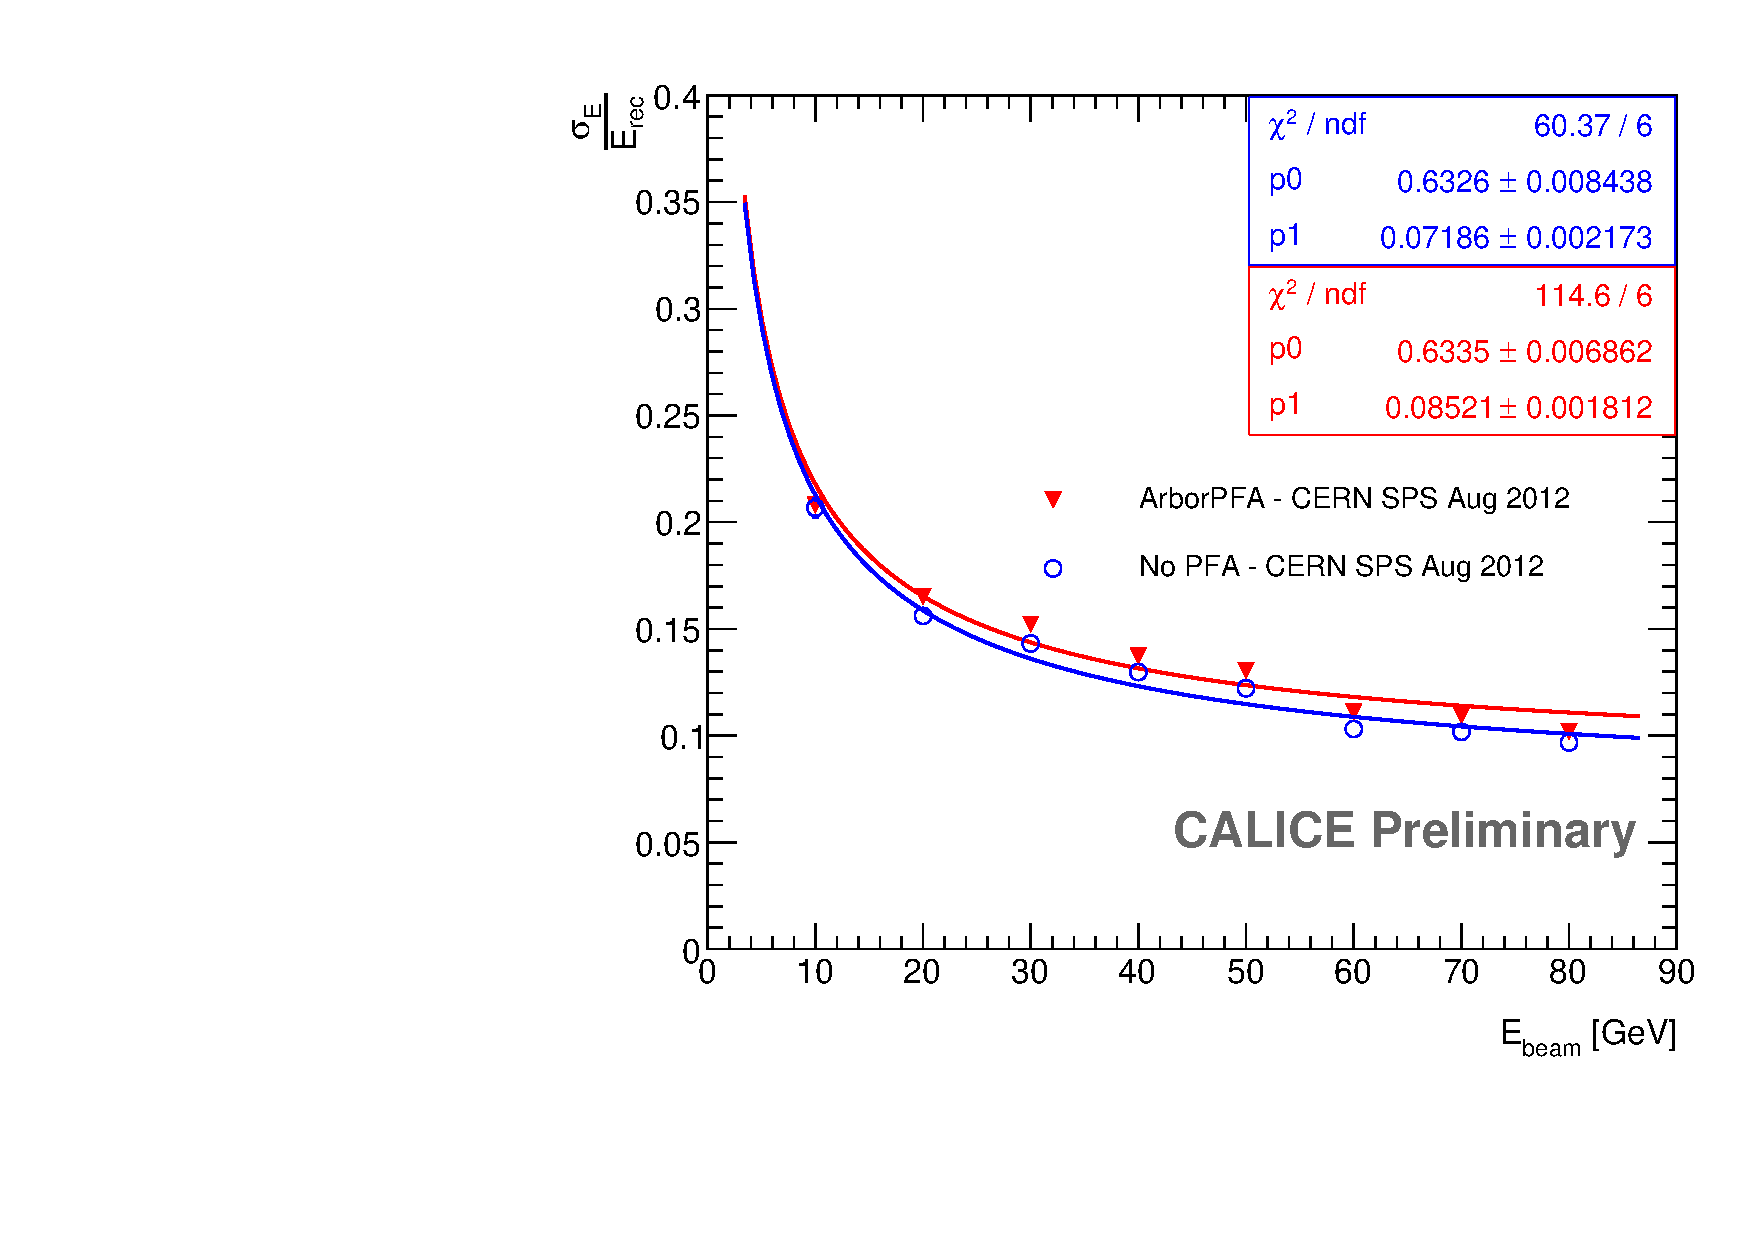
\includegraphics[width=0.48\textwidth]{plots/SingleParticle_EResol.pdf} \\
  \end{center}
  \caption{\label{ARBOR_SINGLE_PARTICLE_EREC_AND_ERESOL} Reconstructed energy (left) and energy resolution (right) before (blue) and after (red) ArborPFA reconstruction on single pion shower event with the SDHCAL prototype}
\end{figure}

The linearity is shown below the reconstructed energy and is defined as :

\begin{equation}
  \Delta E/E_{beam} = \Big(E_{rec} - E_{beam}\Big)/E_{beam}
\end{equation}

These points are extracted using two fits of the energy distributions i) a first gaussian distribution fit over the full reconstructed distribution is performed. The mean $\mu_{E,first}$ and the width $\sigma_{E,first}$ are extracted and ii) a second gaussian fit is performed over the range [$\mu_{E,first}$-1.5*$\sigma_{E,first}$ ; $\mu_{E,first}$+1.5*$\sigma_{E,first}$]. From the last fit we extract the final values of the reconstructed energy and energy resolution defined as the mean $\mu_E$ and the width $\sigma_E$ respectively of the gaussian fit (same procedure applied in \cite{sdhcal-paper}). The efficiency plot has shown that some hits are missing after reconstruction so it is expected to have a small energy decrease in the reconstructed energy. Nevertheless, the linearity is still within 5\% as before applying the reconstruction.

%%%%%%%%%%%%%%%%%%%%%%%%%%%%%%%%%%%%%%%%%%%%%%%%%%%%%
%%%%%% Separation of close-by hadronic showers %%%%%%
%%%%%%%%%%%%%%%%%%%%%%%%%%%%%%%%%%%%%%%%%%%%%%%%%%%%%
\newpage
\section{Separation of close-by hadronic showers}

The ability of a particle flow algorithm to disentangle close-by showers is a key point for the reconstruction in detectors such as ILD of the ILC. To study the confusion between neutral and charged hadrons and the ability of the ArborPFA algorithm to disentangle them, we use again the same test beam data of the SDHCAL prototype. Two different pion showers are first overlaid in the same event and the ArborPFA algorithm is run on the overlaid event with the same parameters as for the single particle study. An analysis of the separation is then performed in order to extract the performance of the algorithm.

\subsection{Overlay procedure and setup}

In order to study the separation of close-by hadronic showers, events from test beam data are overlaid in one event. We have chosen to overlay 10 GeV pions and pions with different energies from 10 GeV up to 50 GeV by step of 10 GeV. Different separation distances between the shower entry point from 5 cm up to 30 cm by step of 5 cm were also used. The choice of this energy range is motivated by the fact that it is the typical single particle energies foreseen at the ILC within jets \cite{ilc-tdr}.

\begin{figure}[!h]
  \begin{center}
    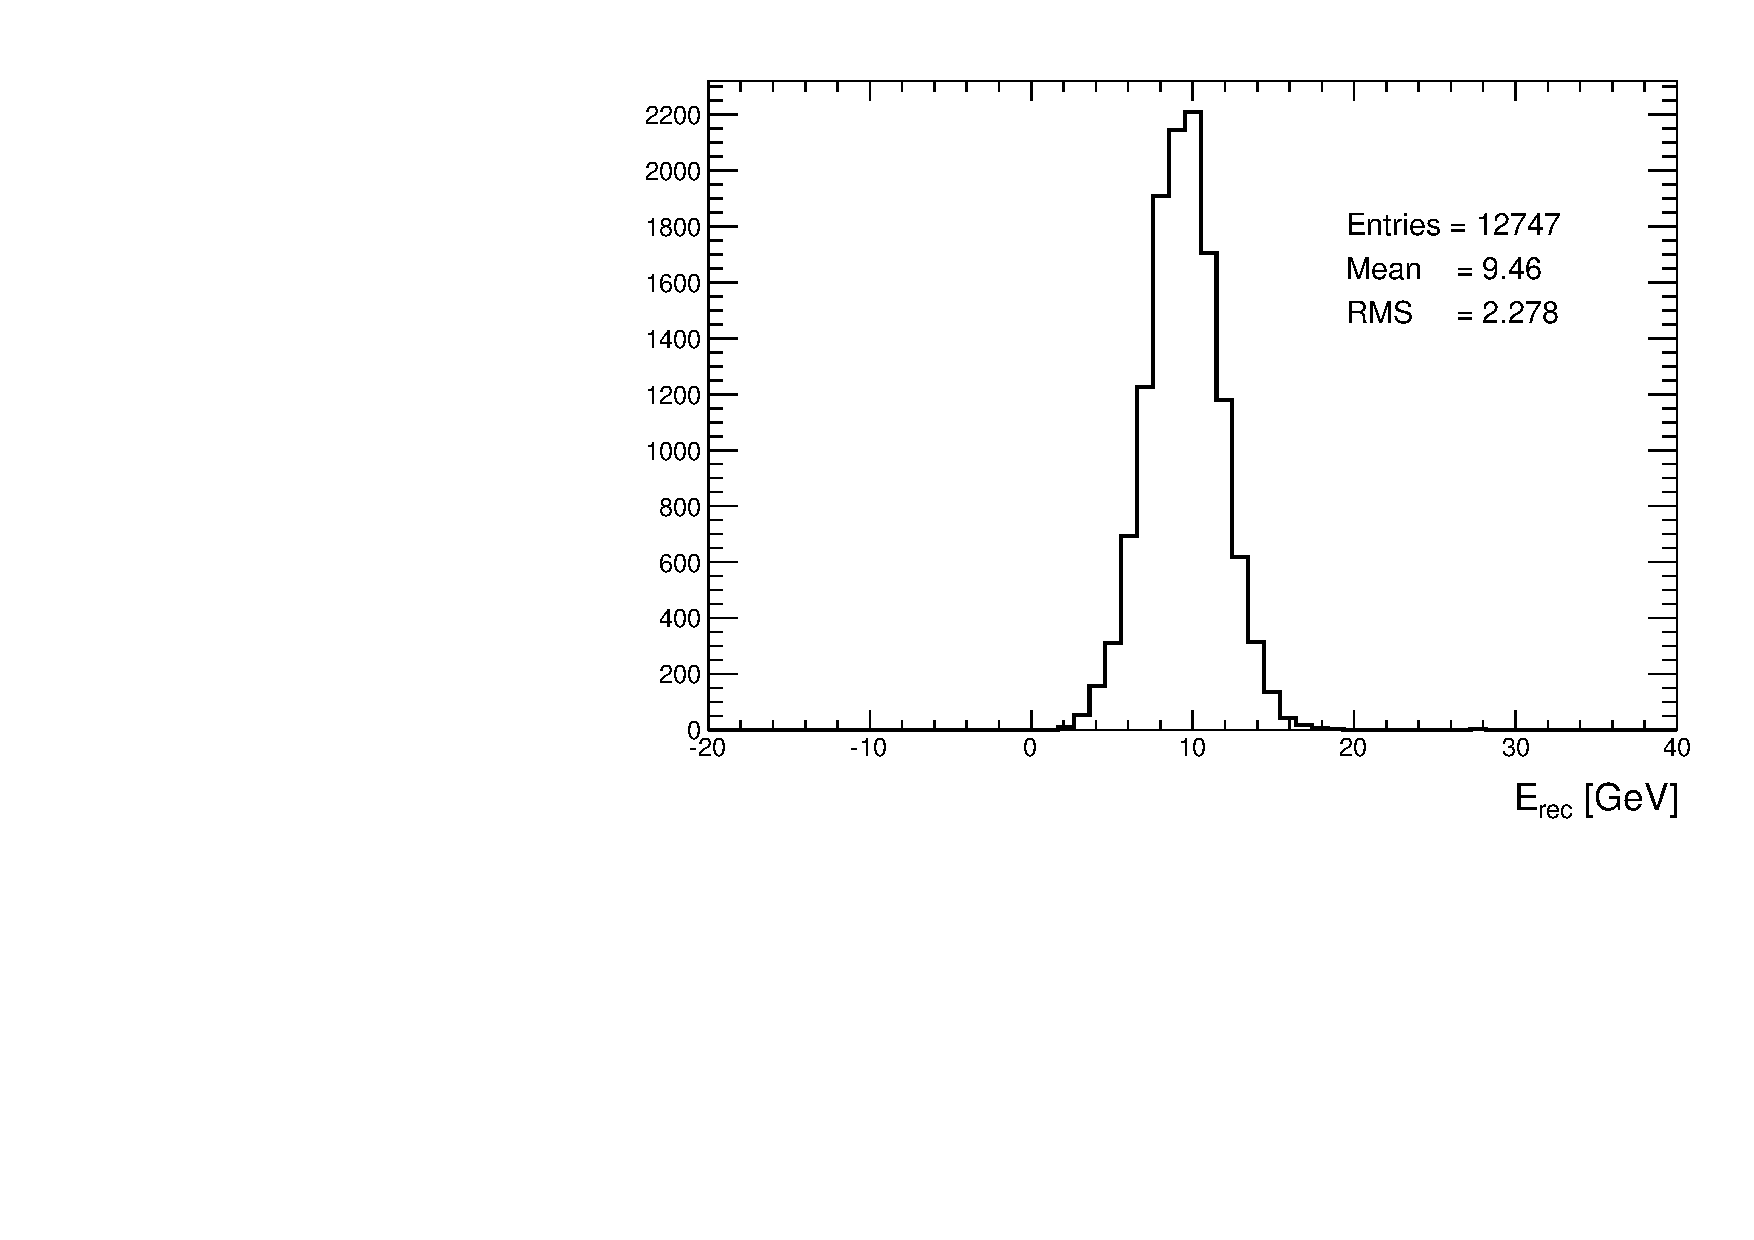
\includegraphics[width=0.47\linewidth]{plots/histo_neutral_mcenergy_ArborPFA_TestBeam_10GeV_n_50GeV_ch_30_cm.pdf}
    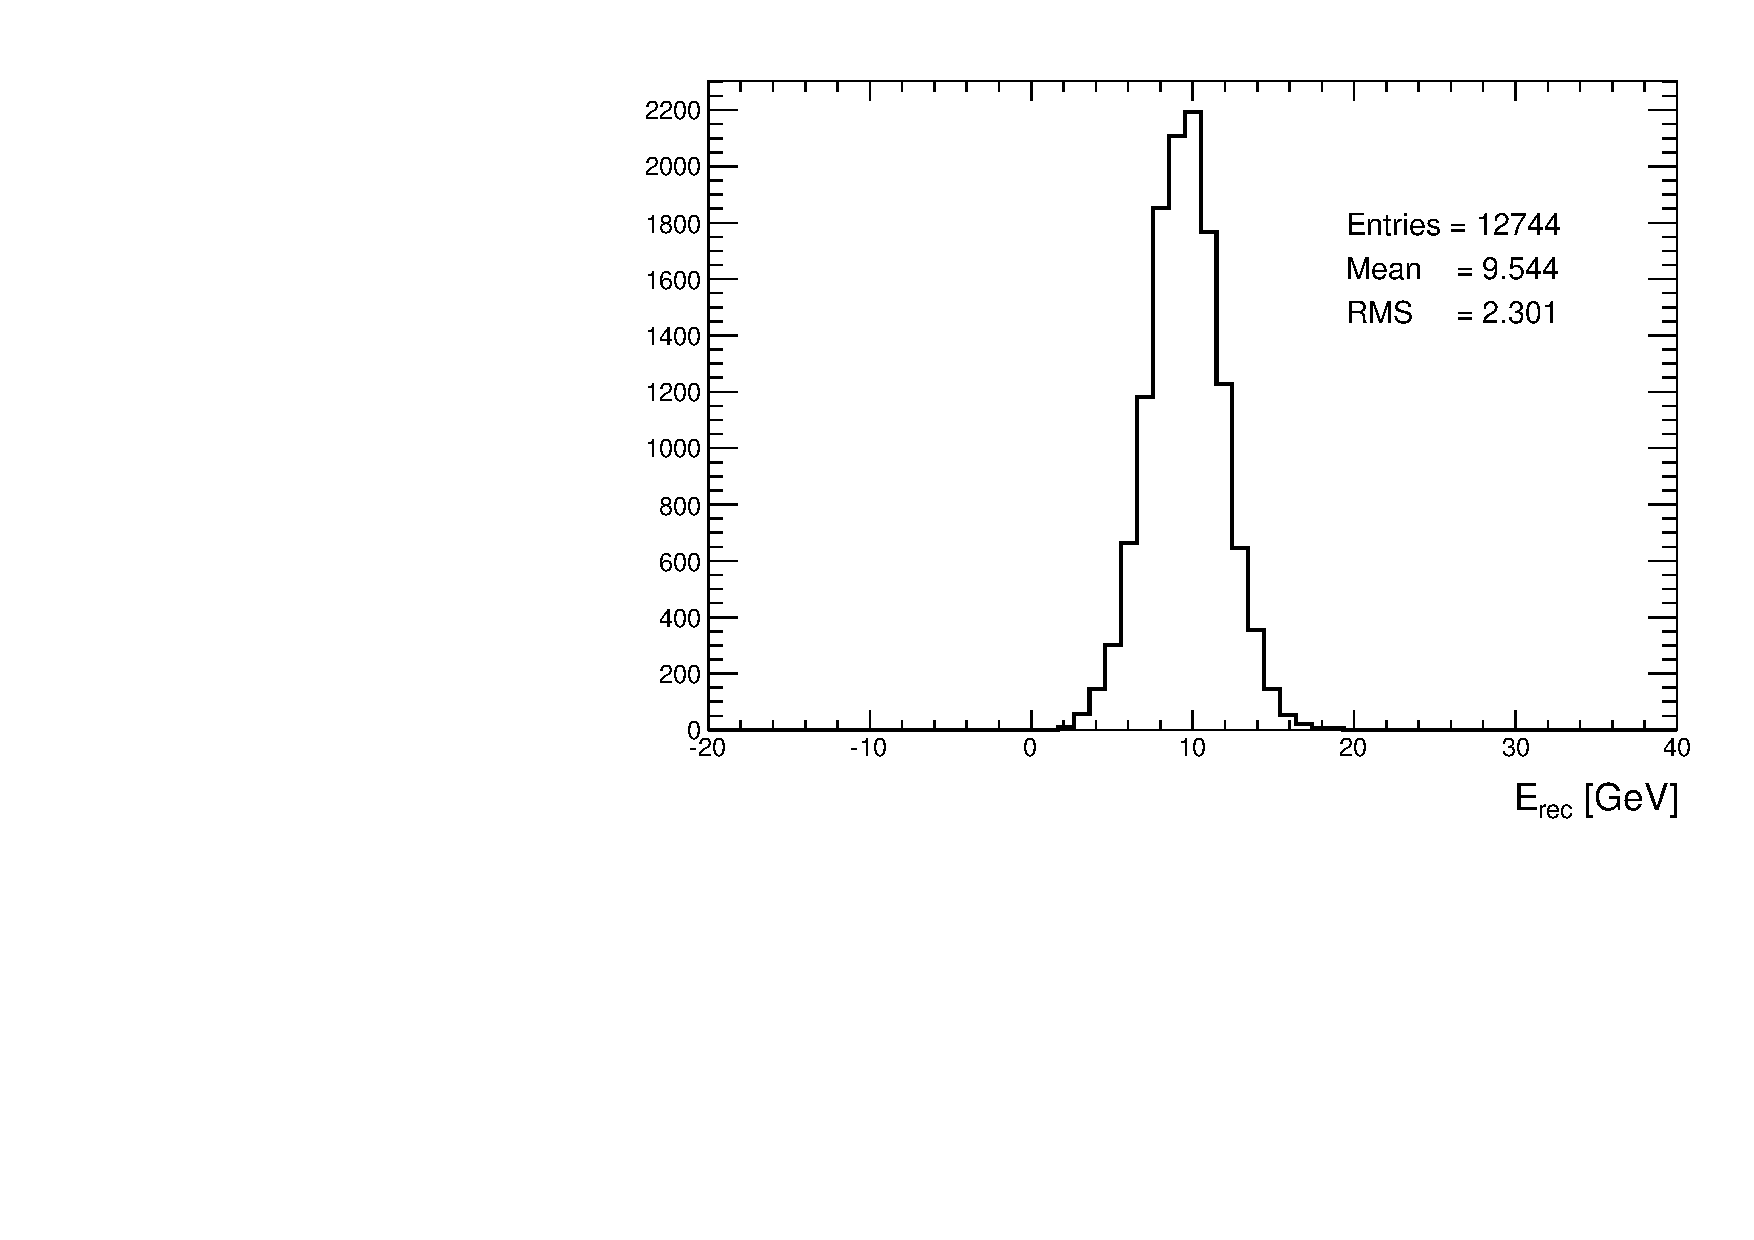
\includegraphics[width=0.47\linewidth]{plots/histo_neutral_mcenergy_ArborPFA_TestBeam_10GeV_n_50GeV_ch_5_cm.pdf}
  \end{center}
  \caption{\label{OVERLAY_EVENT_MC_EREC_OVERLAID_HITS} The reconstructed energy of the 10 GeV neutral hadron after the overlay procedure with a 50 GeV charged hadron with a separation distance of 30 cm (left) and 5 cm (right)}
\end{figure}

The overlay event algorithm is processed as follow :

\begin{enumerate}
  \item The entering track segments of the two showers are determined as for the single particle case. This allows to identify the shower entering points and starting points.
  \item For one of the two pion showers, the hits belonging to its track segments, if any, are removed from the event in order to emulate a neutral hadron shower.
  \item The two showers are then centred along the X and Y axis at the center of the calorimeter. No shift is performed on the Z direction (beam line).
  \item The showers are then shifted along the X axis by a distance of -d/2 for the neutral hadron and +d/2 for the charged particle.
  \item The two events are then overlaid in the same one. At this step a problem may occur : while mixing the showers in the event, pair of hits may overlap in the same cell. Knowing that we are using a semi digital readout and that the information of the deposit charge in each cell is not available in the data, we need to assign a new threshold by using an approximation. The most intuitive one is to keep the highest threshold of the two hits. Figure \ref{OVERLAY_EVENT_MC_EREC_OVERLAID_HITS} shows the reconstructed energy of the 10 GeV neutral hadron overlaid with a 50 GeV charged hadron at 30 cm distance (left) and 5 cm distance (right). The latter case is the worst one that can appears in this study given the energy points and the distances we have chosen. By comparing the two plots, we can see that the effect of this approximation on the reconstructed energy is negligible.
  \item The hits are tagged with respect to our initial showers. All the hits of the neutral hadron are tagged 1 while for the charged hadron the hits are tagged 2. The overlaid hits are tagged 3 so that the information on the overlaid hits can be retrieved after reconstruction.
  \item A new event is created containing the overlaid showers and the entering point of the charged particle track after shifting as shown on figure \ref{OVERLAY_EVENT_DISPLAY}.
\end{enumerate}

\begin{figure}[!h]
  \begin{center}
    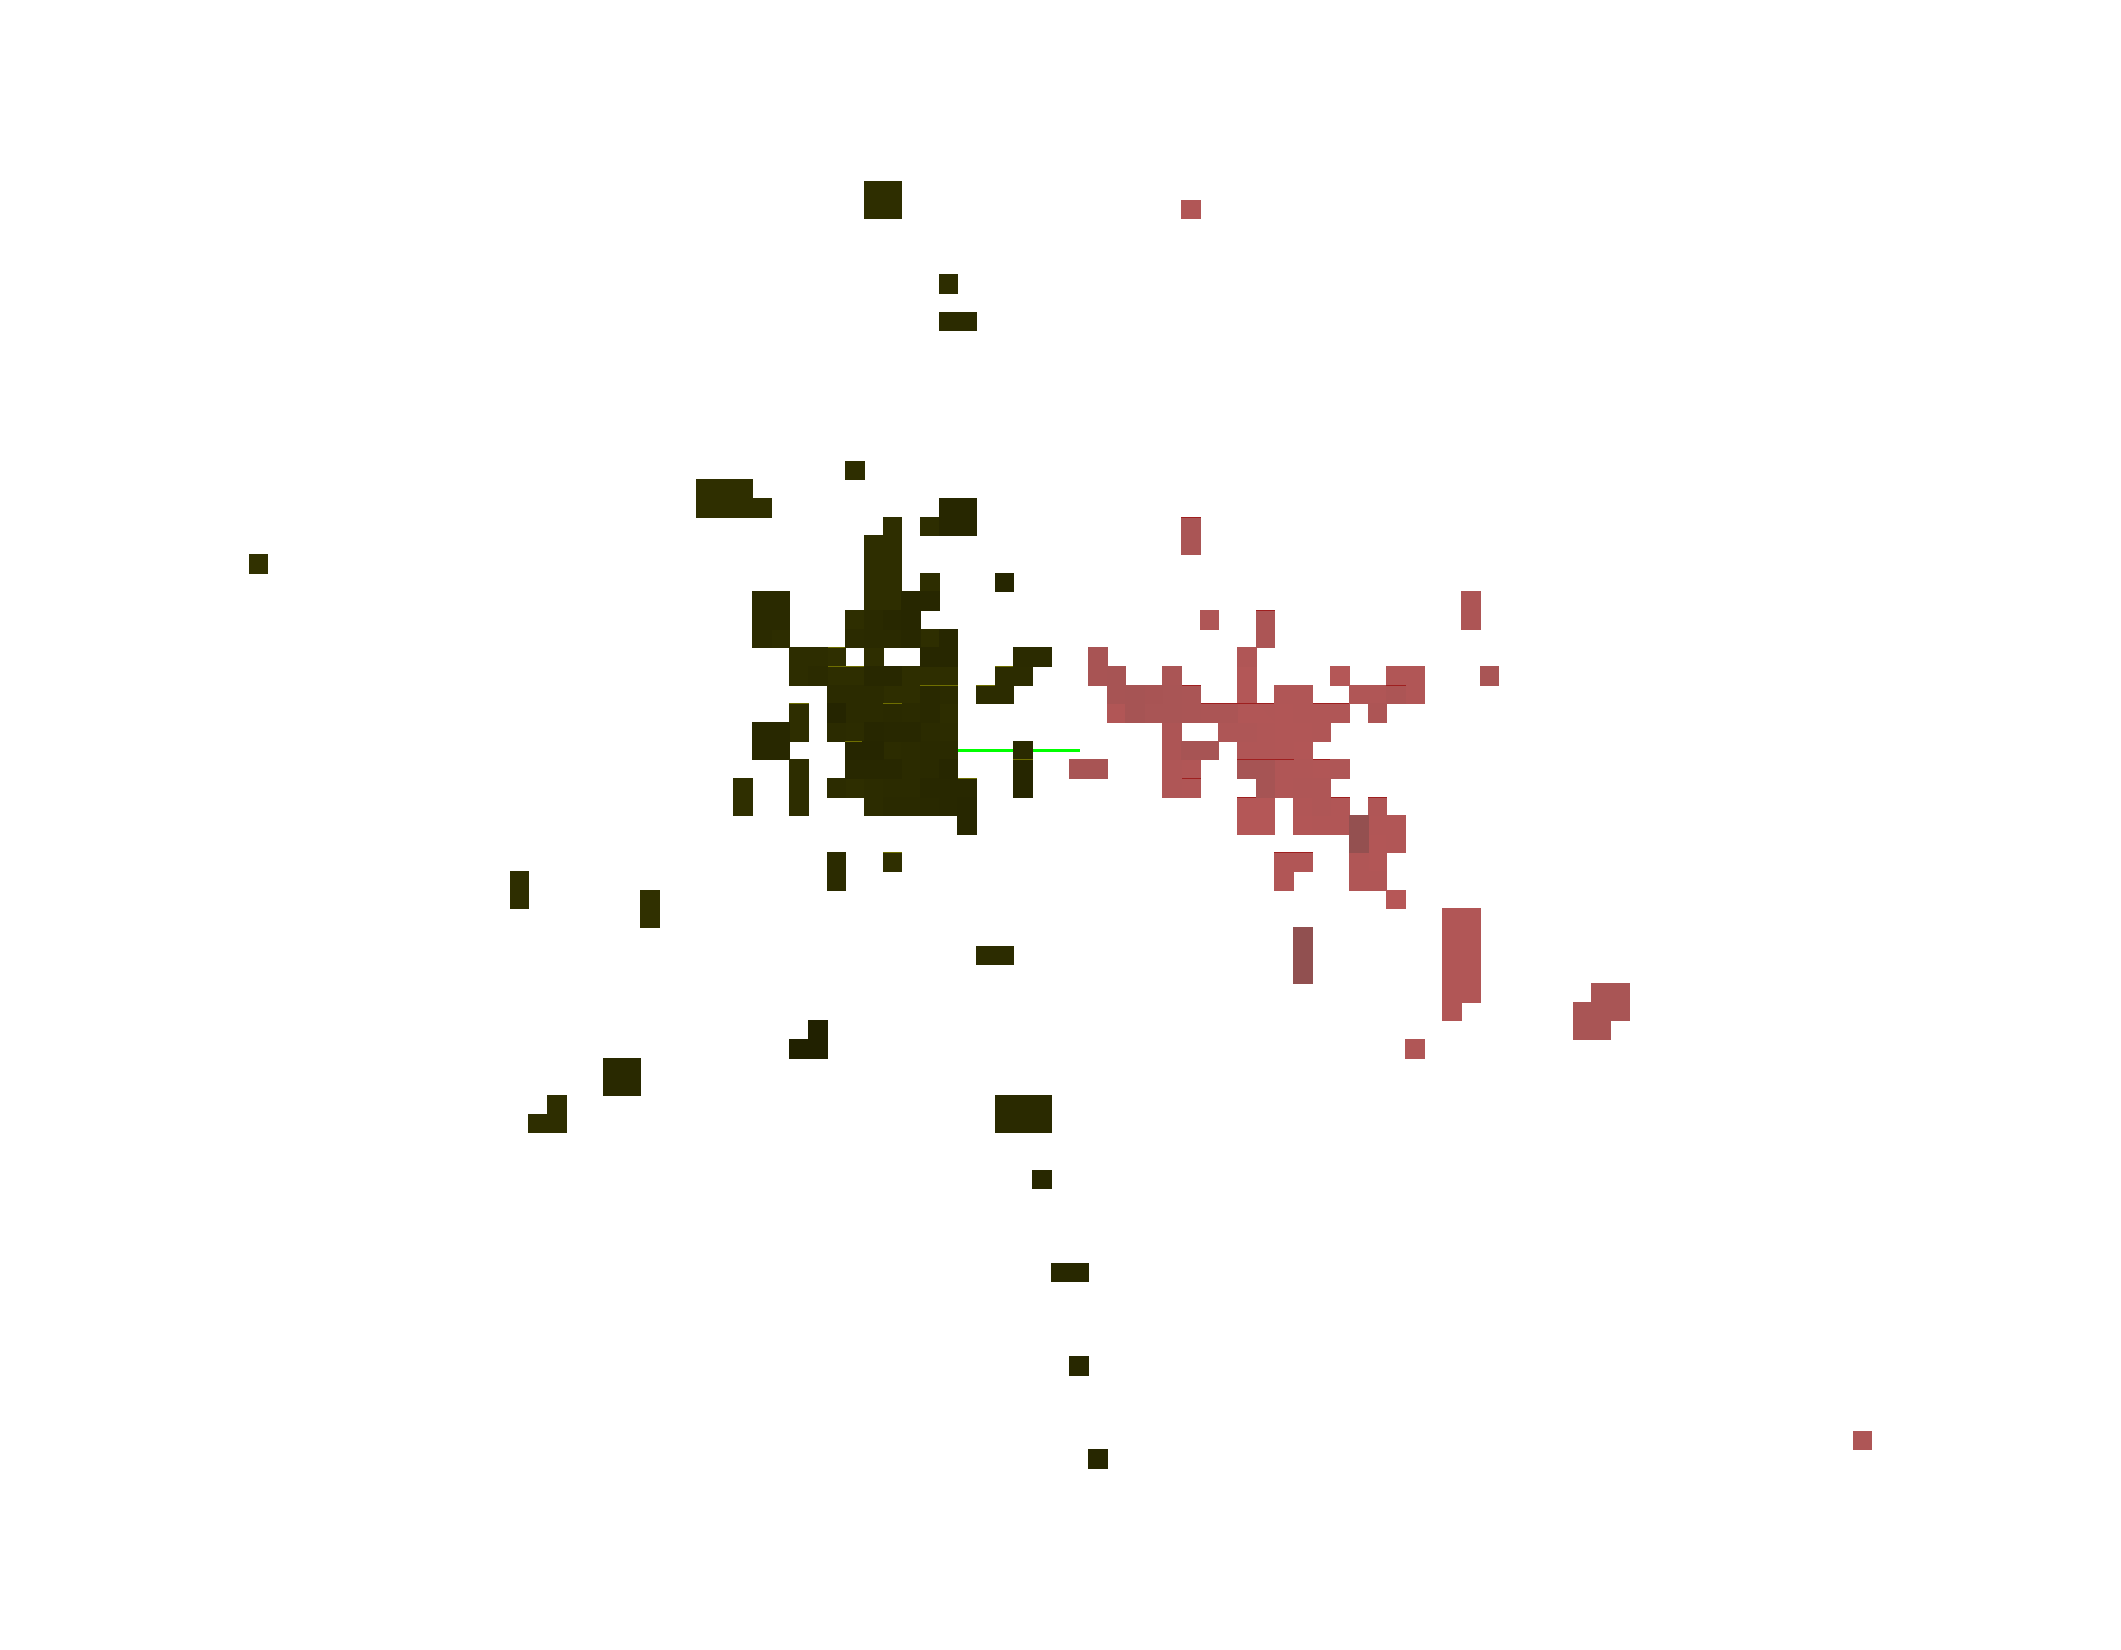
\includegraphics[width=0.32\linewidth]{ArborPFA_PandoraMonitoring_SDHCAL_Overlay_XY.pdf}
    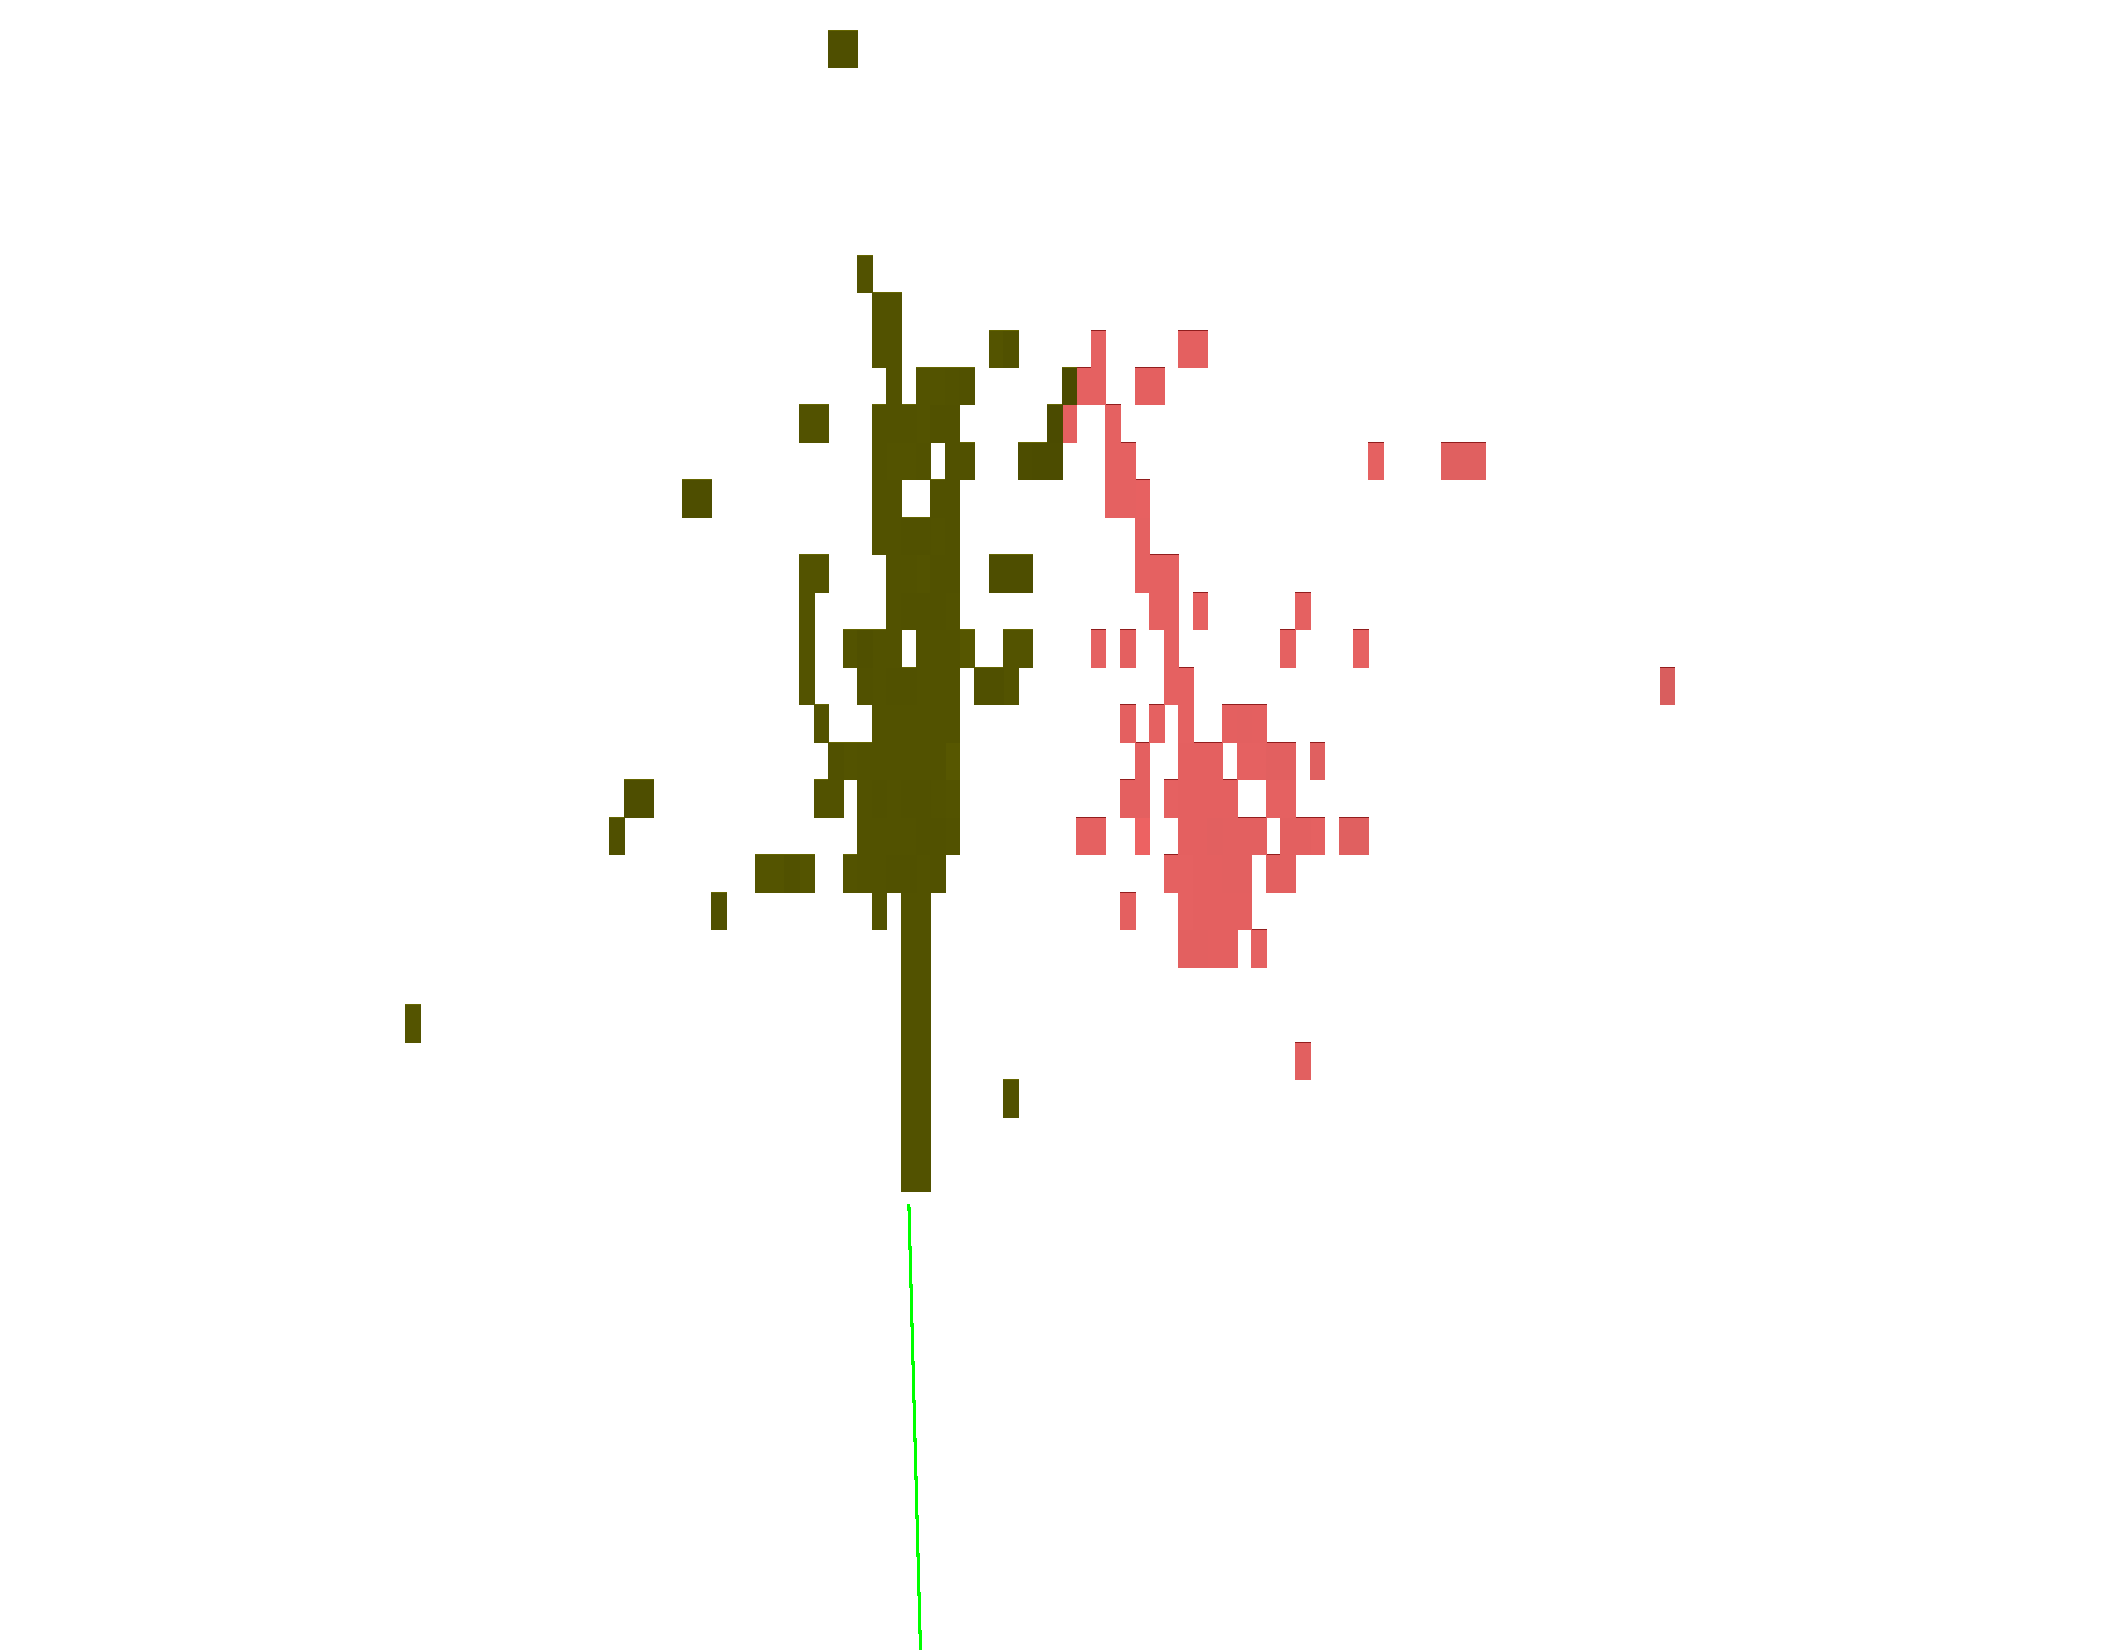
\includegraphics[width=0.32\linewidth]{ArborPFA_PandoraMonitoring_SDHCAL_Overlay_XZ.pdf}
    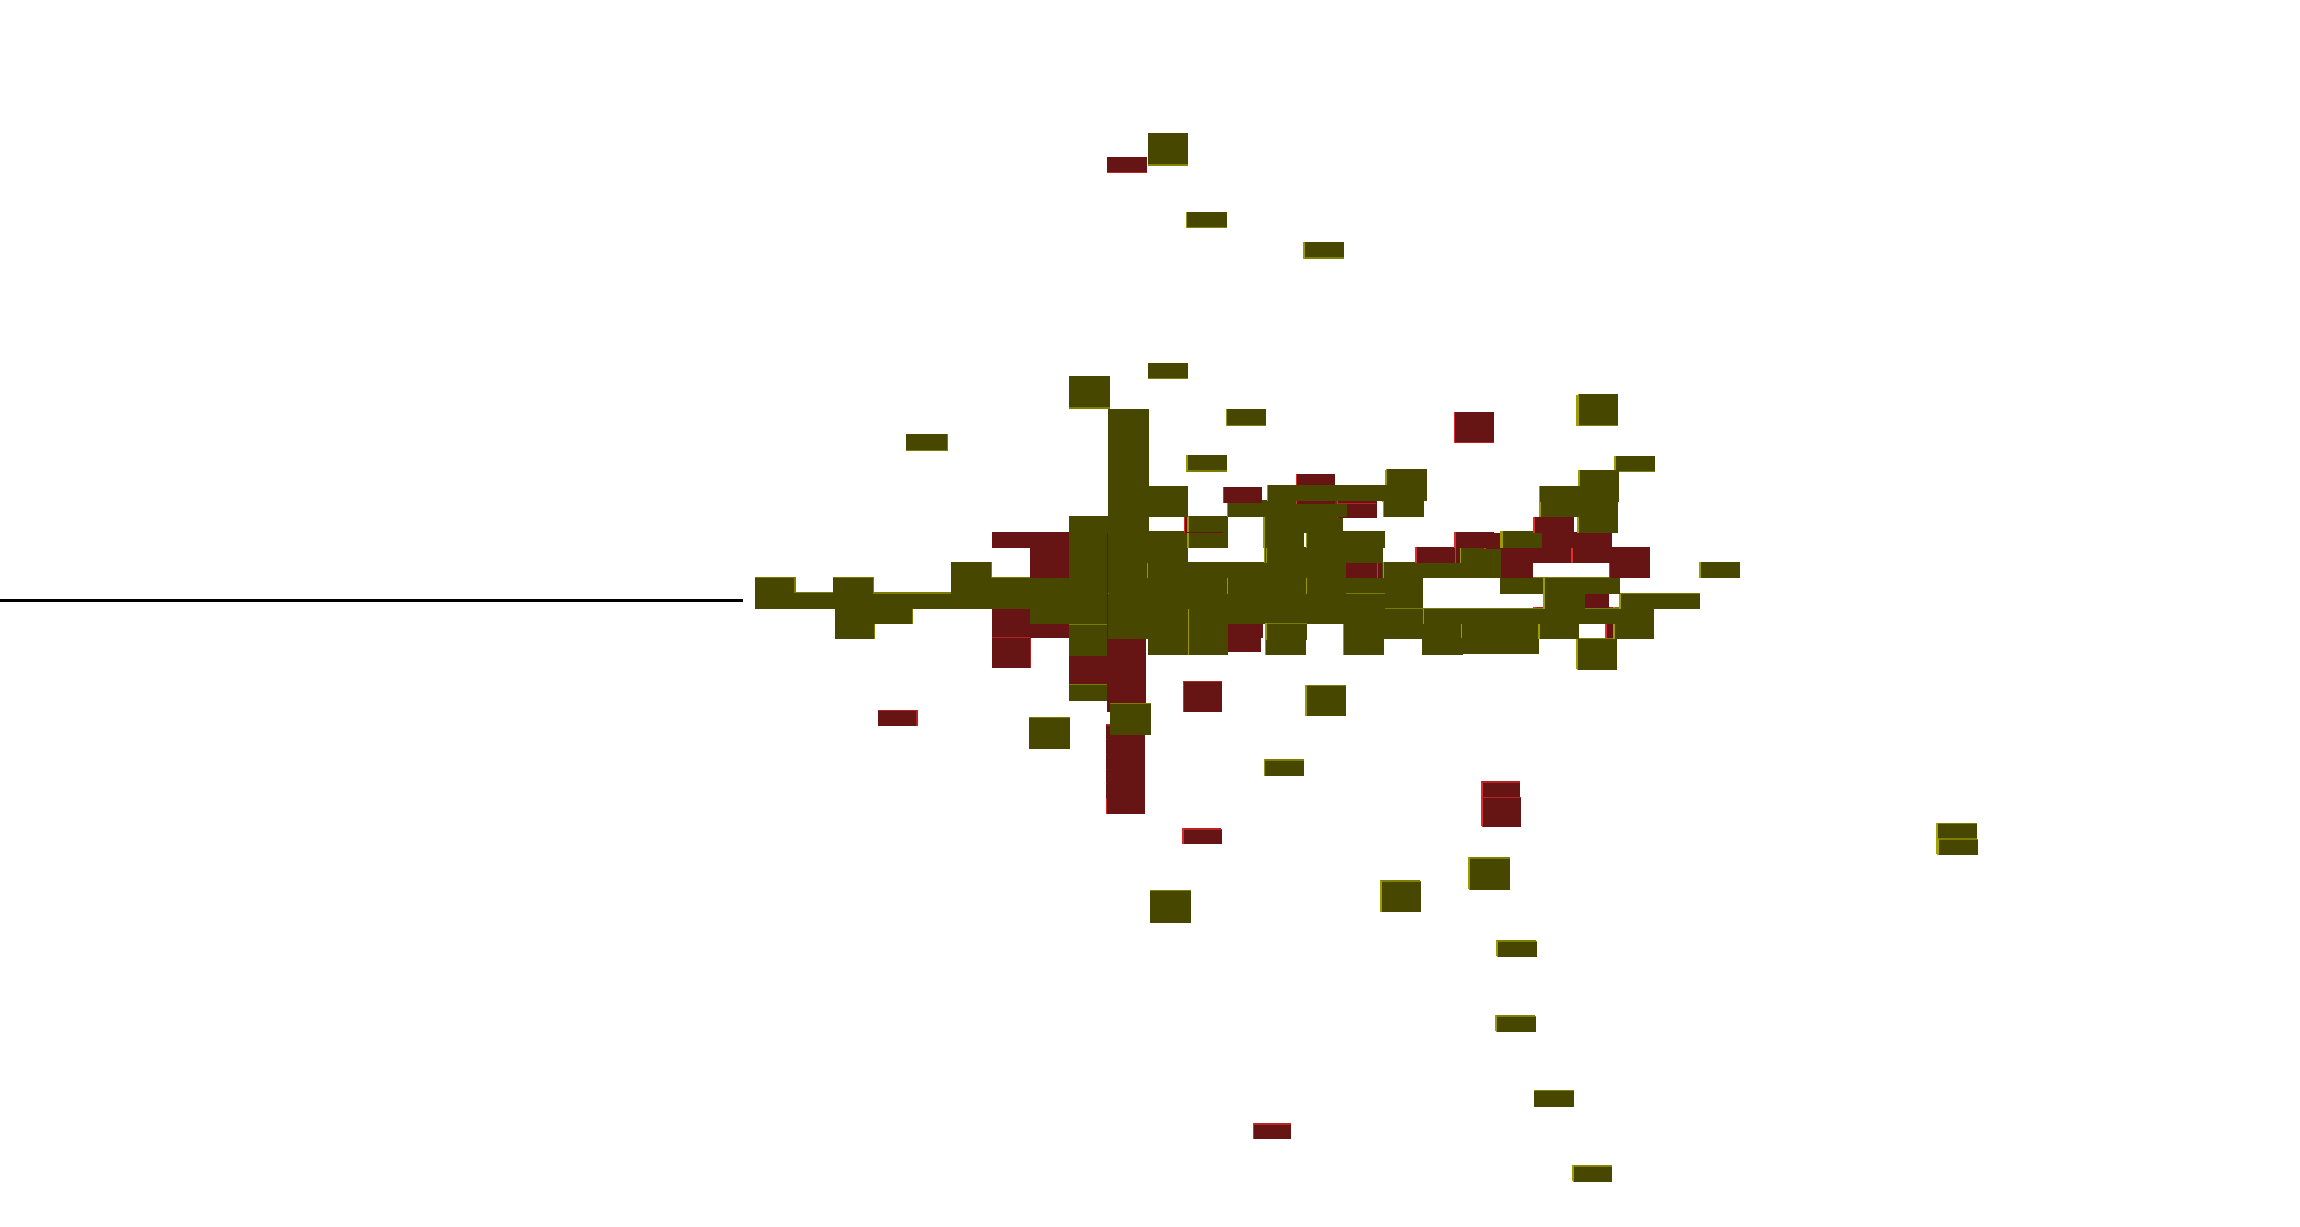
\includegraphics[width=0.32\linewidth]{ArborPFA_PandoraMonitoring_SDHCAL_Overlay_YZ.pdf}
  \end{center}
  \caption{\label{OVERLAY_EVENT_DISPLAY} Event display of a 10 GeV neutral hadron overlaid with a 30 GeV charged hadron at 20 cm separation distance on three different views (XoY on left, XoZ in center and YoZ on right). Colours corresponds to the reconstructed PFOs after running the ArborPFA program. The green straight line is the track generated in front of the calorimeter.}
\end{figure}

\subsection{Overlaid particles analysis}

\begin{figure}[!h]
  \begin{center}
    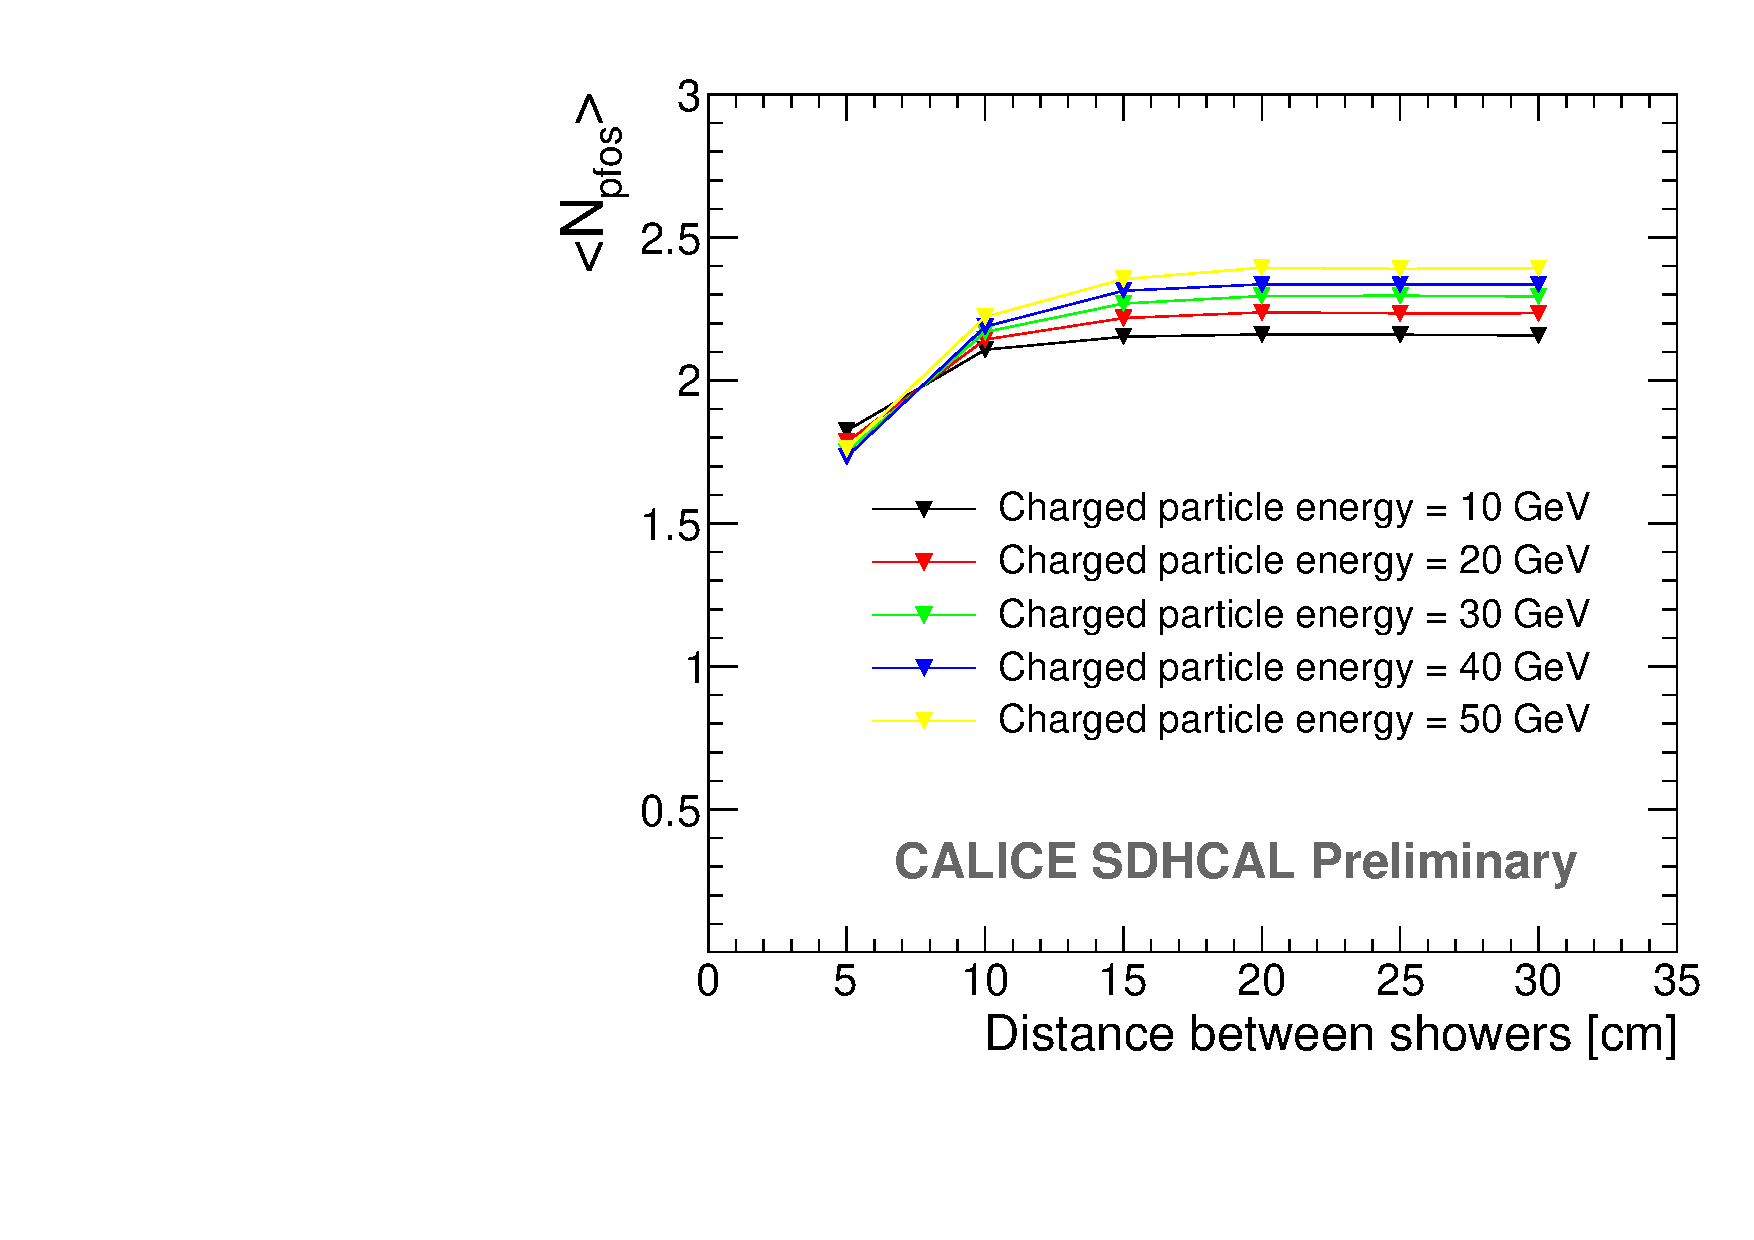
\includegraphics[width=0.6\linewidth]{plots/OverlayEvent_NPfos.pdf}
  \end{center}
  \caption{\label{OVERLAY_EVENT_NPFOS} The mean number of PFOs after running the ArborPFA program on overlaid particles.}
\end{figure}


Figure \ref{OVERLAY_EVENT_NPFOS} shows the mean number of PFOs after running the ArborPFA program on a 10 GeV neutral hadron overlaid with a charged hadron of different energies and different separation distances between them. The behaviour at a large separation distances where the number of PFOs increases with the charged particle energy matches the behaviour of the number of PFOs in the single particle study. We can check that the sum of the number of PFOs for the single particle is compatible with the number of PFOs for the overlay. We can see that the mean number of PFOs is stable at large separation distances but decreases for distances shorter than 10 cm from 2.1 PFOs down to 1.8 PFOs due to the showers overlap and confusions.

\begin{figure}[!h]
  \begin{center}
    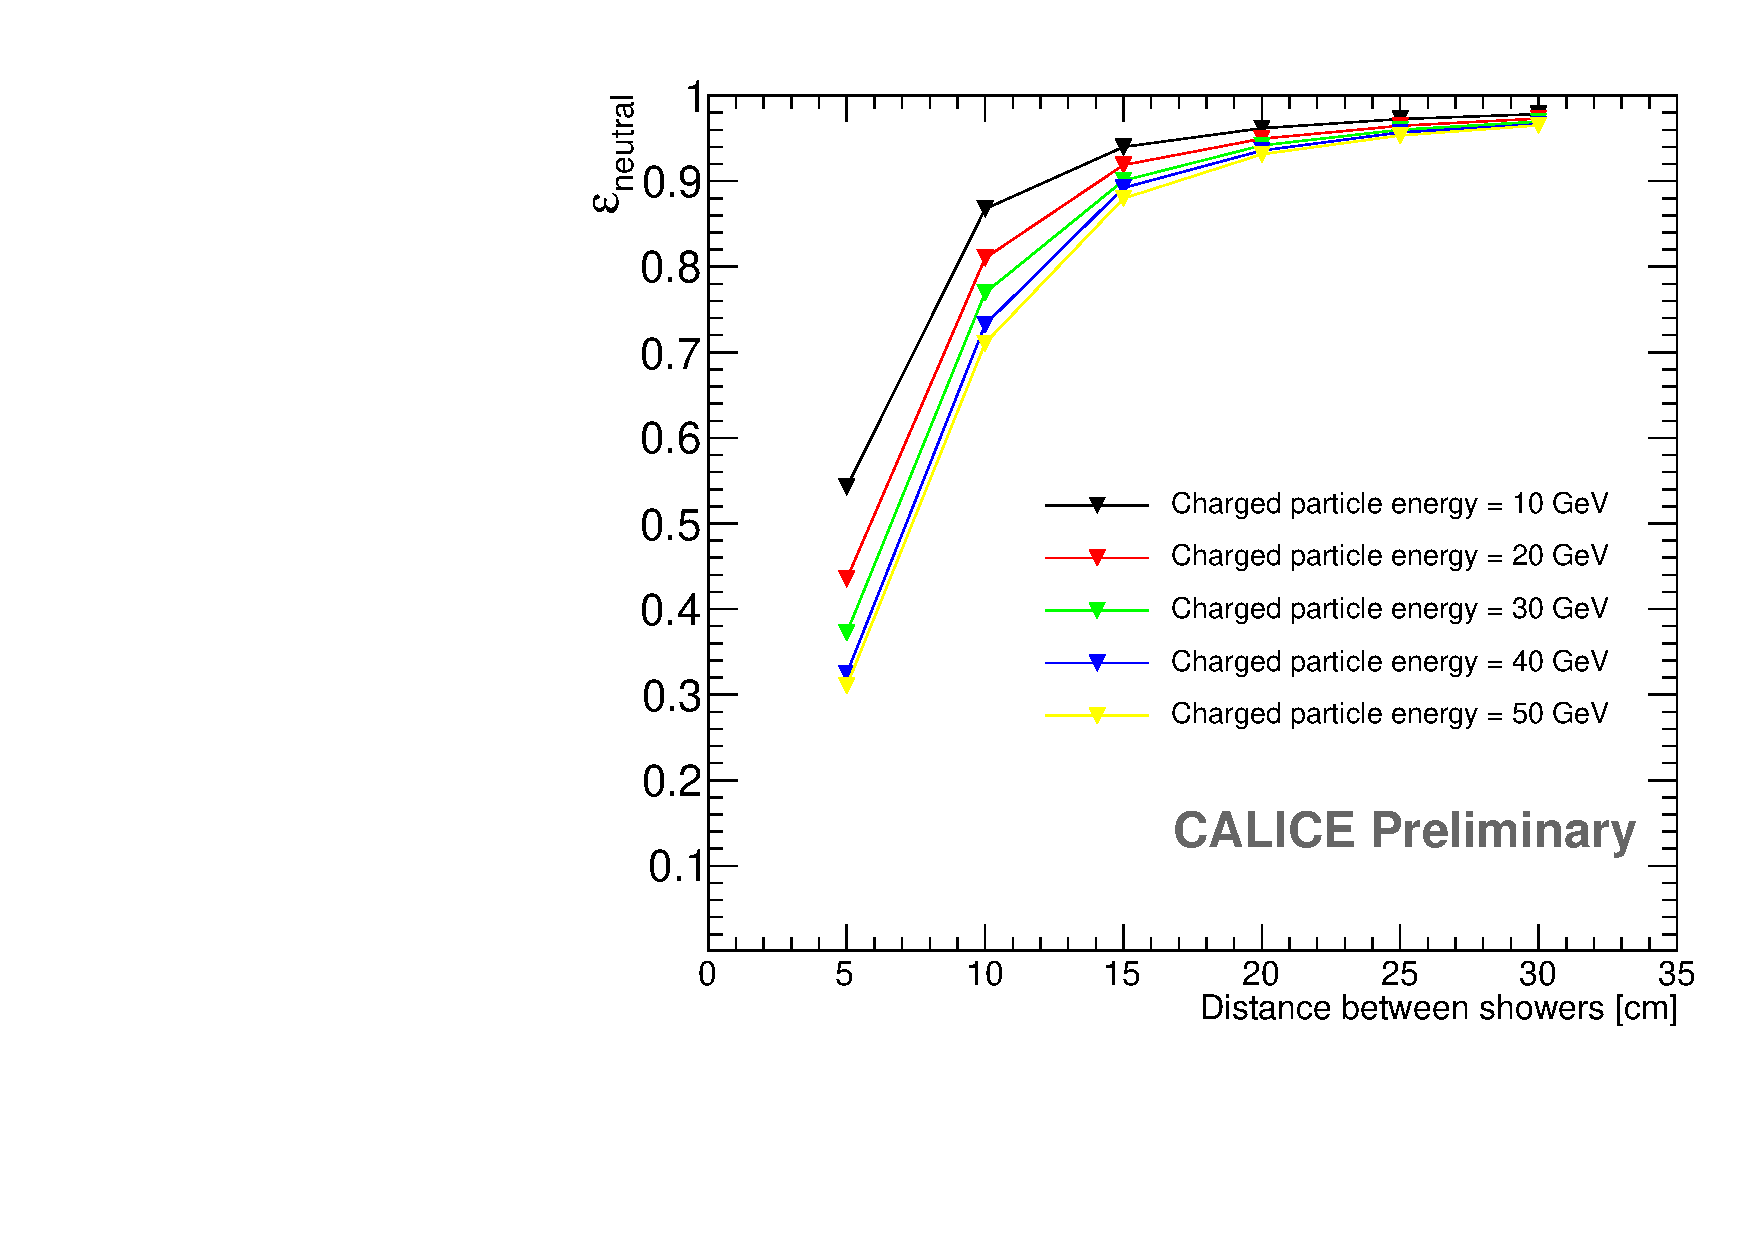
\includegraphics[width=0.47\linewidth]{plots/OverlayEvent_NeutralEfficiency.pdf}
    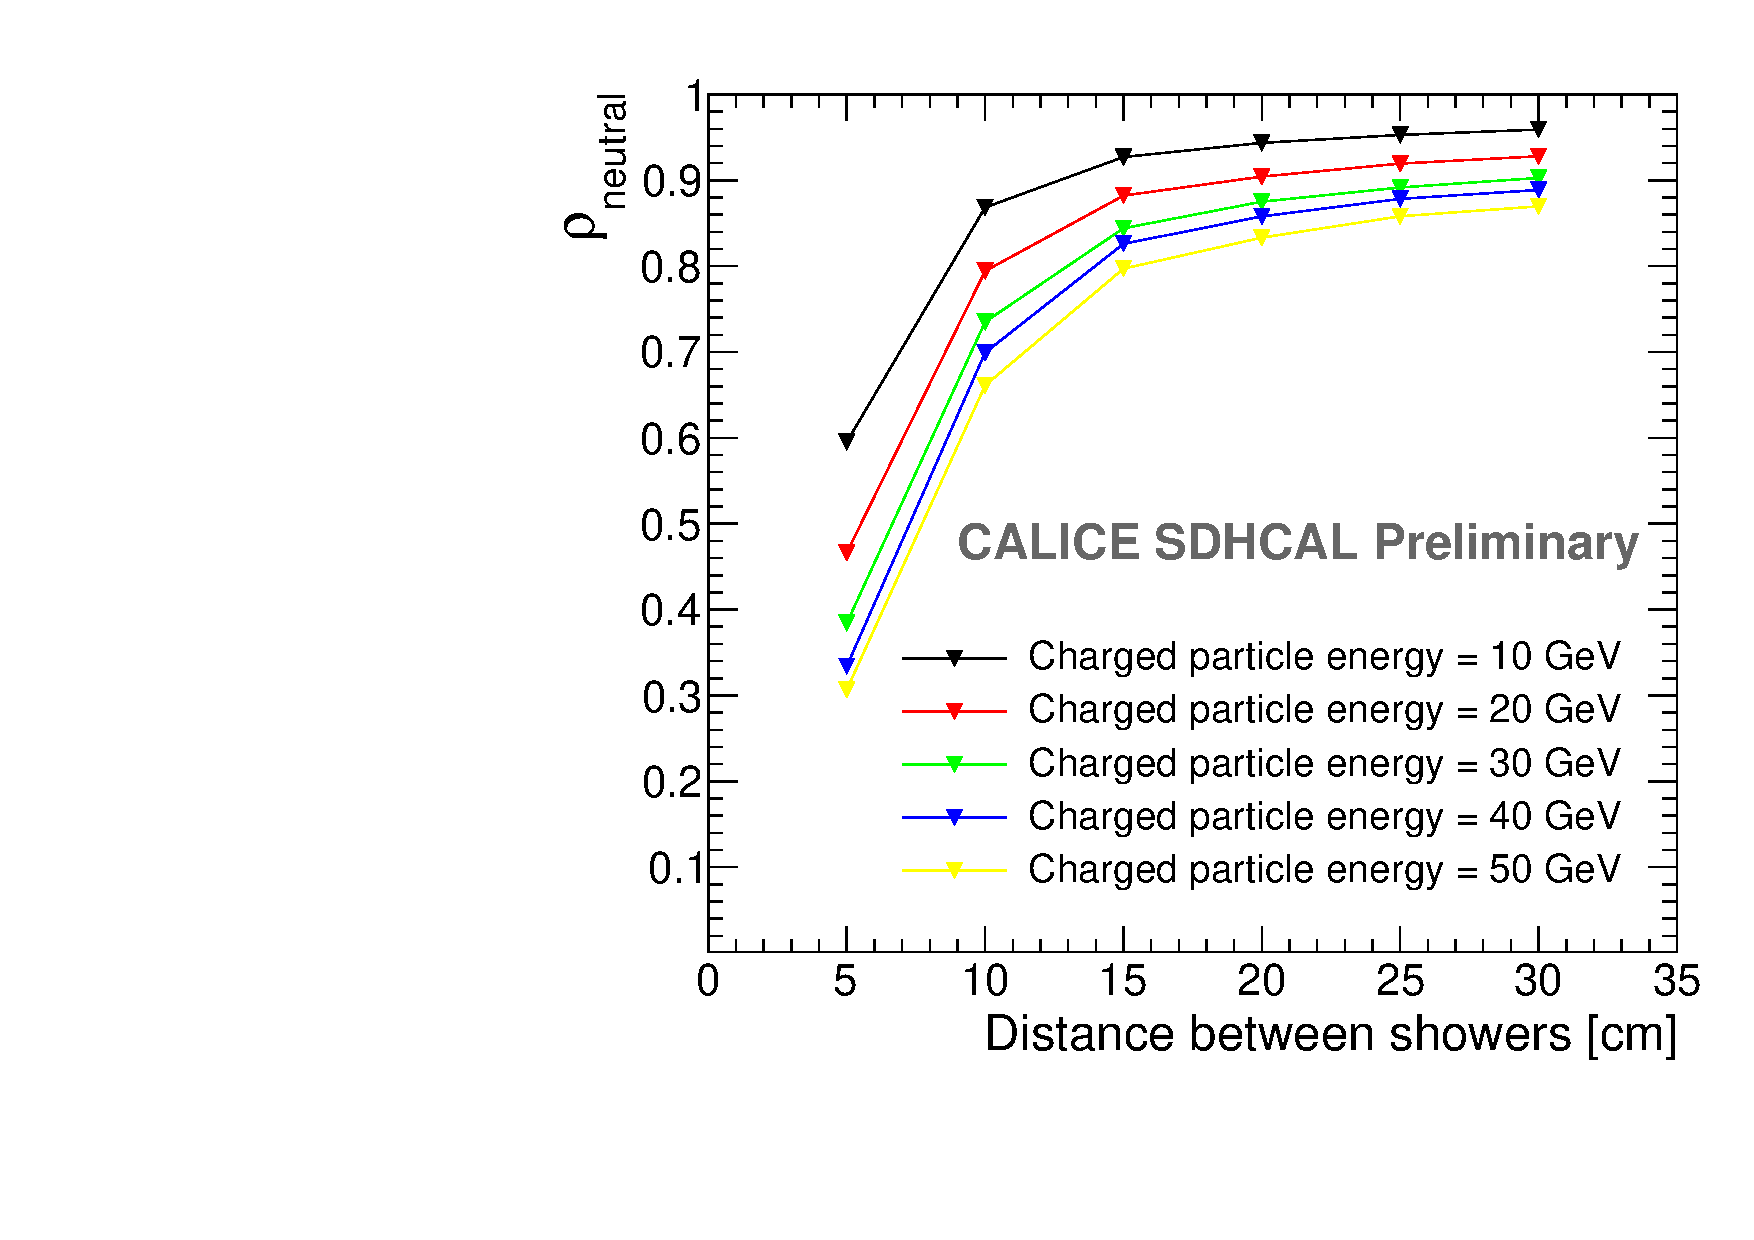
\includegraphics[width=0.47\linewidth]{plots/OverlayEvent_NeutralPurity.pdf}
  \end{center}
  \caption{\label{OVERLAY_EVENT_PURITY_EFFICIENCY} The efficiency (left) and purity (right) of the 10 GeV neutral hadron after separation with a charged hadron}
\end{figure}


To quantify the separation, we define the efficiency and the purity related to the reconstruction of one of the two related showers as :

\begin{equation}
  \epsilon = \frac{Nhit_{good}}{NHit_{ini,tot}}
\end{equation}
\begin{equation}
  \rho = \frac{Nhit_{good}}{Nhit_{rec,tot}}
\end{equation}

with Nhit$_{good}$ the number of hits that initially belong to the particle and correctly assigned after reconstruction, Nhit$_{rec,tot}$ the total number of hits of the reconstructed shower and Nhit$_{ini,tot}$ the total number of hits of the particle before reconstruction. 

Figure \ref{OVERLAY_EVENT_PURITY_EFFICIENCY} shows the efficiency (left) and the purity (right) of the neutral hadron for different charged particle energies and different separation distances. As for the mean number of PFOs, at small distances the two showers start to overlap and confusions appear while the reconstruction is performed. Thus, some hits of the neutral hadron are assigned to the charged one (and vice versa) and the efficiency and purity decrease. At large separation distances, the purity does not tend to 100\%. This is due to the last performed algorithm (small neutral fragment algorithm) which tends to merge the small neutral cluster fragments in their closest parent cluster, without taking care of the parent cluster size or energy. Since the number of neutral fragments for a single hadron particle increases with the energy, a non-negligible part of the charged hits is assigned to the neutral hadron, leading to a decrease of its purity.

Figure \ref{OVERLAY_EVENT_NEUTRAL_PERCENTAGE} (on the left) shows the fraction of events where at least one neutral hadron has been reconstructed. As expected, the number of reconstructed neutral particles decreases with the separation distance. From 30 cm down to 15 cm, this fraction is stable and very closed to 100\%. At 10 cm, confusions start appearing and the neutral hadron is sometimes merged in the charged one, leading to a small decrease of this fraction. At 5 cm, we can see that the fraction strongly depends on the charged particle energy and goes from 73\% of reconstructed events for the 10 GeV charged particle case down to 60\% for the 50 GeV charged particle case.

\begin{figure}[!h]
  \begin{center}
    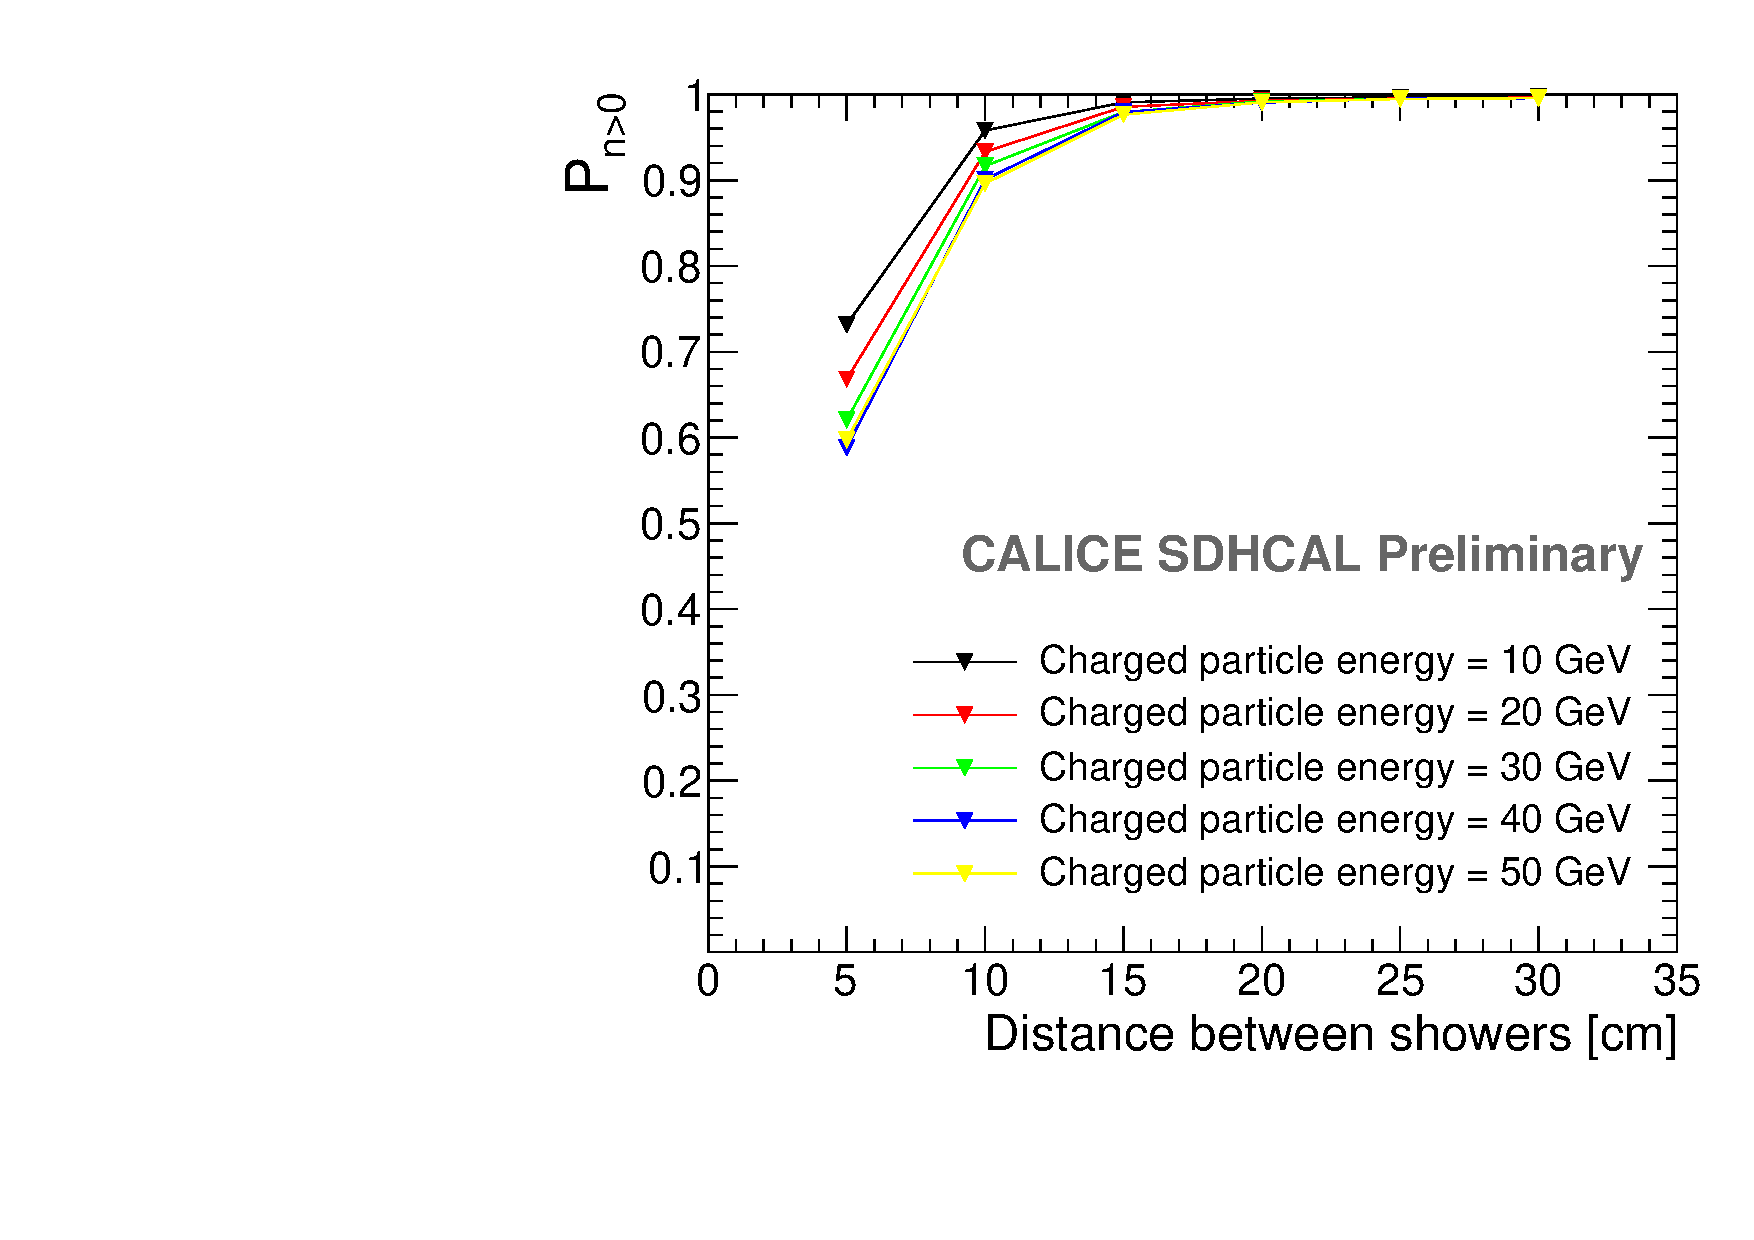
\includegraphics[width=0.47\linewidth]{plots/OverlayEvent_NeutralPercentage.pdf}
    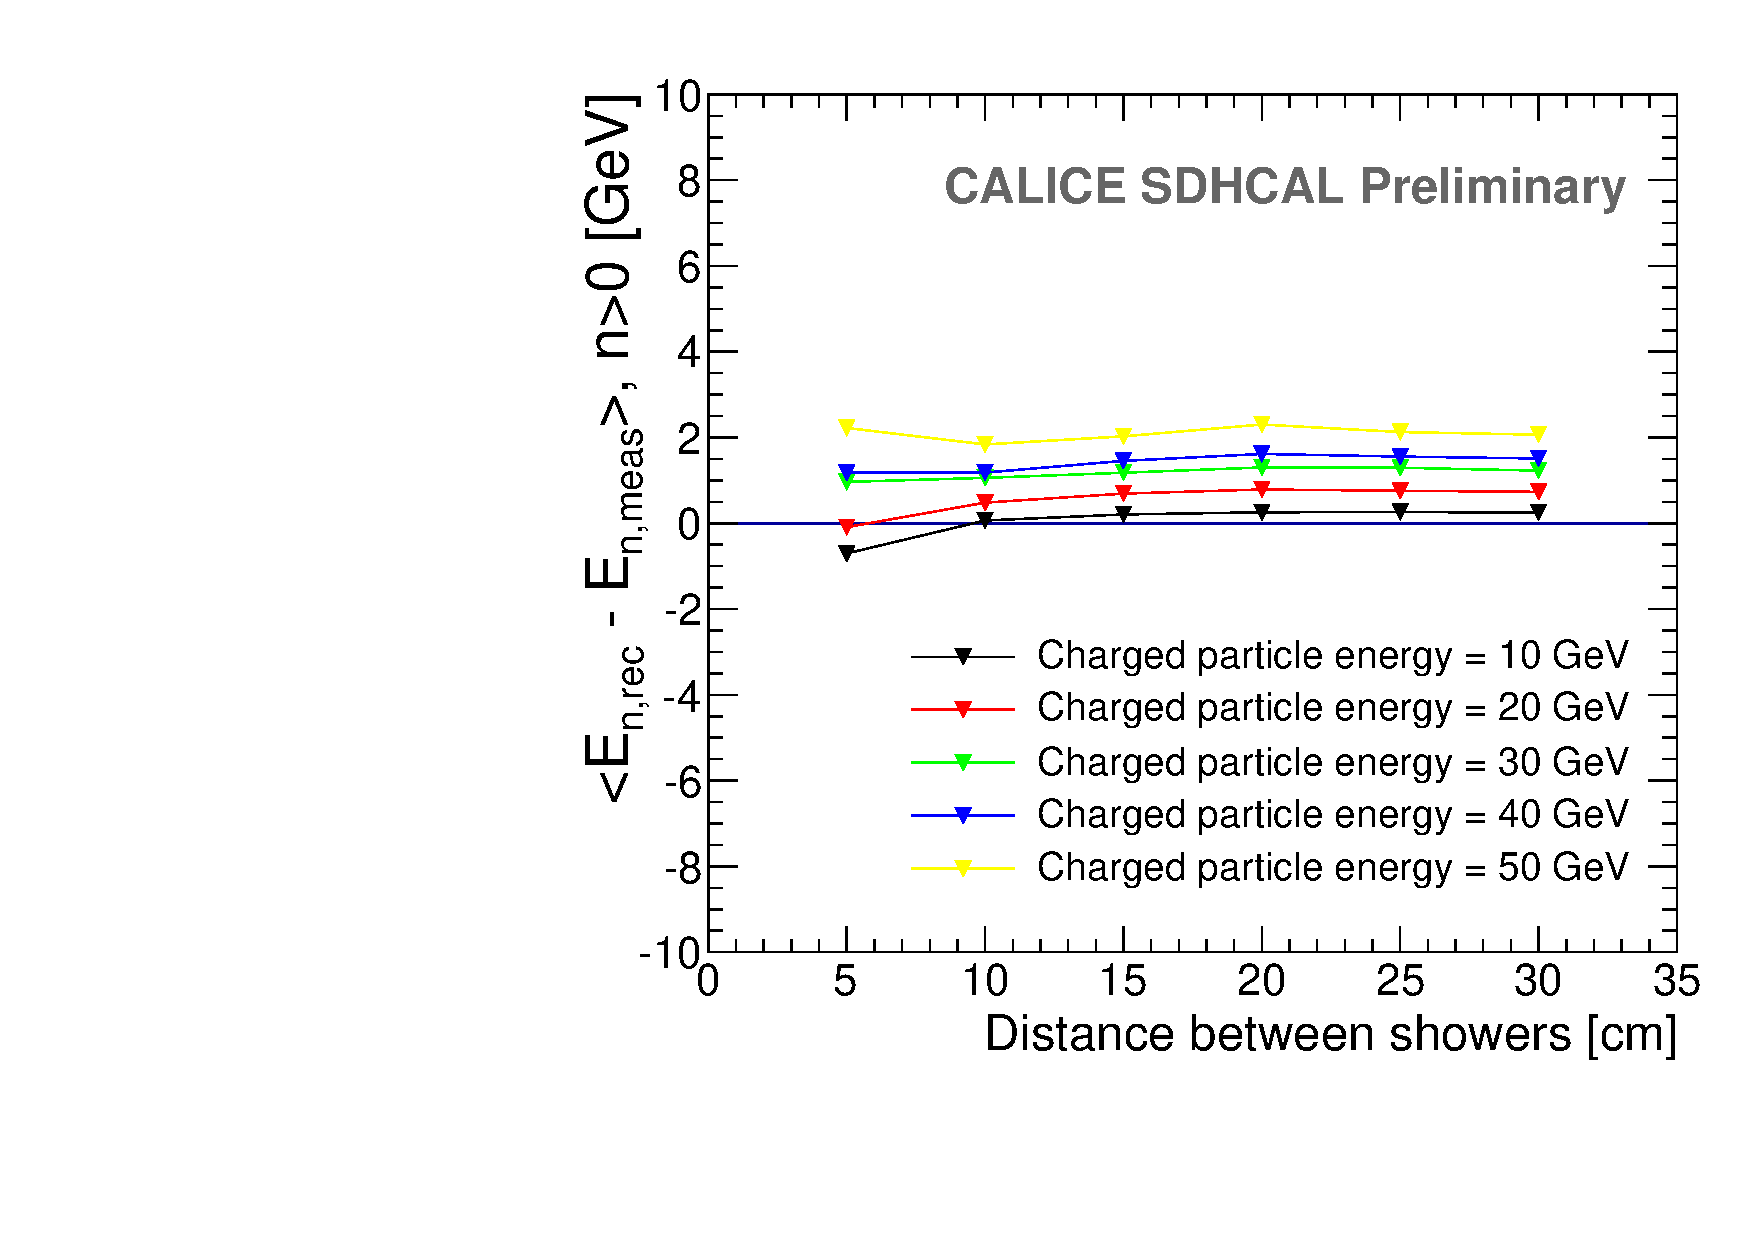
\includegraphics[width=0.47\linewidth]{plots/OverlayEvent_NeutralEnergyDifferenceMeanNeutralEfficient.pdf}
  \end{center}
  \caption{\label{OVERLAY_EVENT_EREC} \label{OVERLAY_EVENT_NEUTRAL_PERCENTAGE} Left : The fraction of events where at least one neutral hadron has been reconstructed. Right : The same variable when at least one neutral hadron has been reconstructed.}
\end{figure}

Figure \ref{OVERLAY_EVENT_EREC} (on the right) shows the mean difference between the reconstructed energy and the measured energy of the neutral hadron in the case where at least on neutral hadron has been reconstructed. As for the purity, the reconstructed energy of the neutral hadron increases with the charged particle energy. This plot also shows a constant evolution of the reconstructed energy with the separation distance. This means that the reconstruction of the neutral hadron at very small distance (5 cm) has a \textit{binary-like} behaviour, either well reconstructed or completely merged in the charged hadron.

%%%%%%%%%%%%%%%%%%%%%
%%%%%% Summary %%%%%%
%%%%%%%%%%%%%%%%%%%%%
\newpage
\section{Summary}

The ArborPFA algorithm has been described in details with all the sub-algorithms. 

A single particle study has been performed on SDHCAL test beam data taken at SPS at CERN during August and September 2012 \cite{sdhcal-paper}. Single pion showers have been selected and a track in front of the calorimeter has been created in order to emulate a TPC track.

The results showed a good efficiency with more than 95\% of hits assigned to the reconstructed charged particle over the whole energy range. The mean number of PFOs shows an increase with the energy from 1.1 PFOs at 10GeV up to 1.4 PFOs at 80 GeV growing linearly. The reconstructed energy of the single charged hadron is close to the one applied before running the algorithm with a small decrease due to the 5\% of inefficiency and thus the energy resolution increases too.

The algorithm has also been applied in order to separate close-by hadronic showers. Two different charged hadron showers with different energies from the same test beam data set have been overlaid in the same event with different separation distances. For one of the two showers the mip track inside the calorimeter has been identified and removed from the event in order to emulate a neutral hadron particle. For the other particle, a track has been generated in front of the calorimeter and pointing on the particle entry point, as for the single particle case. 

The results showed a good neutral hadron efficiency and purity until 10 cm separation distance where a non negligible confusion starts to appear. 

The difference between the reconstructed energy and the measured energy of the neutral hadron in the case where at least one neutral hadron has been reconstructed showed an increase with the charged hadron energy for all the separation distances due to the small neutral fragment merging algorithm. At small separation distance (5cm), the difference stays constant and shows taht the neutral hadron reconstruction has a \textit{binary-like} behaviour, either a very good reconstruction or merged in the charged hadron.

This work will be extended shortly to include the electromagnetic calorimeter as well as the other sub-detectors in the framework of the ILD detector with the aim to separate charged and neutral hadrons produced in jets to improve on the PFA performances.

\newpage
\begin{thebibliography}{6}
\renewcommand{\hepex}[1]{\href{http://www.arxiv.org/abs/#1}{\tt hep-ex/#1}}
\renewcommand{\physics}[1]{\href{http://www.arxiv.org/abs/#1}{\tt phys.int-det/#1}}
\newcommand\nim[4]{\href{http://dx.doi.org/10.1016/#4}
  {\emph{Nucl.\ Instrum.\ Meth.} {\bf #1} (#2) #3}}
\newcommand\can[1]{\href{https://twiki.cern.ch/twiki/pub/CALICE/CaliceAnalysisNotes/CAN-#1.pdf}{\tt CAN-#1}}


\bibitem{sdhcal-paper} 
Calice Collaboration, \emph{First results of the CALICE SDHCAL technological prototype}, \can{037}

\bibitem{ilc-tdr} 
J. Carwardine {\it et al.},  \emph{International Linear Collider Technical Design Report}. 1) Executive Summary, 2) Physics, 3) Accelerator, 4) Detectors. 12 June 2013

\bibitem{marlin-lccd}
F. Gaede, Marlin and LCCD: Software tools for the ILC, Nucl.Instrum.Meth. A559 (2006) 177-180

\bibitem{pandora-pfa}
M. A. Thomson, \emph{Particle Flow Calorimetry and the PandoraPFA Algorithm}, \physics{0907.3577}

\bibitem{pandora-sdk}
J. S. Marshall, M. A. Thomson, \emph{The Pandora Software Development Kit for Pattern Recognition}, \physics{1506.05348}


\bibitem{arbor-manqi}
M. Ruan, \emph{Arbor, a new approach of the Particle Flow Algorithm}, Proceeding of CHEF 2013. \hepex{1403.4784}


\bibitem{ilcsoft}
ILCsoft, 2012. \href{http://ilcsoft.desy.de/portal}{\tt http://ilcsoft.desy.de/portal}


\bibitem{root}
ROOT, 1995-2015, \href{https://root.cern.ch/drupal}{\tt https://root.cern.ch/drupal}

\newpage

\end{thebibliography}


\clearpage
\appendix

\section{ArborPFA algorithm parameters}
\label{ARBOR_ALGORITHM_PARAMETERS}

% Object creation
\paragraph{Object creation algorithm} ~

\begin{table}[!h]
  \begin{center}
    \begin{tabu} to \linewidth { c | c } 
          Parameter name & value \\
          \hline
          MaxClusterSize & 4 \\
          IntraLayerDistance & 11 mm
    \end{tabu} 
  \end{center}
\end{table}

\begin{itemize}
 \item MaxClusterSize \\
 $\rightarrow$ The maximum intra layer cluster size to build an object with. Else the object is split in single calo hit objects
 \item IntraLayerDistance \\
 $\rightarrow$ The nearest neighbour intra layer clustering maximum distance
\end{itemize}


% Track segment candidate tagging
\paragraph{Track segment candidate tagging algorithm} ~

\begin{table}[!h]
  \begin{center}
    \begin{tabu} to \linewidth { c | c } 
          Parameter name & value \\
          \hline
          MaxNNeighbors & 6 \\
          IntraLayerNeighbourDistance ($\Delta_{mip}$) & 50 mm
    \end{tabu} 
  \end{center}
\end{table}

\begin{itemize}
  \item MaxNNeighbors \\
  $\rightarrow$ The maximum number of neighbouring objects within a layer
  \item IntraLayerNeighbourDistance ($\Delta_{mip}$) \\
  $\rightarrow$ The maximum distance between two neighbours in a layer used for the neighbour counting
\end{itemize}

\newpage
% Primary track connection
\paragraph{Primary track connection} ~

\begin{table}[!ht]
  \begin{center}
    \begin{tabu} to \linewidth { c | c } 
          Parameter name & value \\
          \hline
          ConnectionDistance & 110 mm \\ 
          BackwardConnectorWeight & 2 \\ 
          ForwardConnectorWeight & 3 \\ 
          OrderParameterAnglePower & 1 \\ 
          OrderParameterDistancePower & 5 \\
          MaxNEmptyConsecutiveLayers & 3 
    \end{tabu} 
  \end{center}
\end{table}

\begin{itemize}
  \item ConnectionDistance \\
  $\rightarrow$ The maximum connection distance used for the primary track connectors creation
  \item BackwardConnectorWeight \\
  $\rightarrow$ The backward connector weight assigned for the reference vector computation
  \item ForwardConnectorWeight \\
  $\rightarrow$ The forward connector weight assigned for the reference vector computation
  \item OrderParameterAnglePower \\ 
  $\rightarrow$ The angle power parameter of the $\kappa$ parameter while cleaning connectors
  \item OrderParameterDistancePower \\
  $\rightarrow$ The distance power parameter of the $\kappa$ parameter while cleaning connectors
  \item MaxNEmptyConsecutiveLayers \\
  $\rightarrow$ The maximum consecutive empty layers to take into account for the connector seeding
\end{itemize}


% Connector seeding 1
\paragraph{Connector seeding 1} ~

\begin{table}[!ht]
  \begin{center}
    \begin{tabu} to \linewidth { c | c } 
          Parameter name & value \\
          \hline
          ConnectionDistance & 45 mm
    \end{tabu} 
  \end{center}
\end{table}

\begin{itemize}
  \item ConnectionDistance \\
  $\rightarrow$ The maximum connection distance used for a connector creation
\end{itemize}


\newpage
% Connector cleaning 1
\paragraph{Connector cleaning 1} ~

\begin{table}[!ht]
  \begin{center}
    \begin{tabu} to \linewidth { c | c } 
          Parameter name & value \\
          \hline
          BackwardConnectorWeight & 2 \\
          ForwardConnectorWeight & 2 \\
          OrderParameterAnglePower & 1 \\
          OrderParameterDistancePower & 5 \\
          ReferenceDirectionDepth & 1
    \end{tabu} 
  \end{center}
\end{table}

\begin{itemize}
  \item BackwardConnectorWeight \\
  $\rightarrow$ The weight of a backward connector assigned in the reference direction vector calculation.
  \item ForwardConnectorWeight \\
  $\rightarrow$ The weight of a forward connector assigned in the reference direction vector calculation.
  \item OrderParameterAnglePower \\
  $\rightarrow$ The $\theta$ angle power parameter used for the $\kappa$ parameter computation
  \item OrderParameterDistancePower \\
  $\rightarrow$ The $\Delta$ distance power parameter used for the $\kappa$ parameter computation
  \item ReferenceDirectionDepth \\
  $\rightarrow$ The forward connector depth used for the reference vector computation
\end{itemize}


% Connector seeding 2
\paragraph{Connector seeding 2} ~

\begin{table}[!ht]
  \begin{center}
    \begin{tabu} to \linewidth { c | c } 
          Parameter name & value \\
          \hline
          ConnectionDistance & 65 mm \\
          ConnectionAngle & 0.7 rad
    \end{tabu} 
  \end{center}
\end{table}

\begin{itemize}
  \item ConnectionDistance \\
  $\rightarrow$ The maximum connection distance used for a connector creation
  \item ConnectionAngle \\
  $\rightarrow$ The maximum angle between two connectors
\end{itemize}


\newpage
% Connector cleaning 2
\paragraph{Connector cleaning 2} ~

\begin{table}[!ht]
  \begin{center}
    \begin{tabu} to \linewidth { c | c } 
          Parameter name & value \\
          \hline
          BackwardConnectorWeight & 0.1 \\
          ForwardConnectorWeight & 5 \\
          OrderParameterAnglePower & 1 \\
          OrderParameterDistancePower & 5 \\
          ReferenceDirectionDepth & 2
    \end{tabu} 
  \end{center}
\end{table}

\begin{itemize}
  \item BackwardConnectorWeight \\
  $\rightarrow$ The weight of a backward connector assigned in the reference direction vector calculation.
  \item ForwardConnectorWeight \\
  $\rightarrow$ The weight of a forward connector assigned in the reference direction vector calculation.
  \item OrderParameterAnglePower \\
  $\rightarrow$ The $\theta$ angle power parameter used for the $\kappa$ parameter computation
  \item OrderParameterDistancePower \\
  $\rightarrow$ The $\Delta$ distance power parameter used for the $\kappa$ parameter computation
  \item ReferenceDirectionDepth \\
  $\rightarrow$ The forward connector depth used for the reference vector computation
\end{itemize}


% Energy driven track cluster association
\paragraph{Energy driven track cluster association} ~

\begin{table}[!ht]
  \begin{center}
    \begin{tabu} to \linewidth { c | c } 
          Parameter name & value \\
          \hline
          TrackToClusterDistanceCut1 & 75 mm \\
          TrackToClusterDistanceCut2 & 55 mm \\
          FirstInteractingLayerNSeedCut & 15 \\
          TrackToClusterNLayersCut & 3 \\
          TrackClusterPsi2Cut & 3 \\
          Psi2SigmaFactor & 1.5
    \end{tabu} 
  \end{center}
\end{table}

\begin{itemize}
  \item TrackToClusterDistanceCut1 \\
  $\rightarrow$ The maximum distance between the track projection at calorimeter front face and a cluster seed. This distance is used to detect an early interacting cluster.
  \item TrackToClusterDistanceCut2 \\
  $\rightarrow$ The reduced maximum distance between the track projection at calorimeter front face and a cluster seed. This distance is used when no early interacting cluster has been detected.
  \item FirstInteractingLayerNSeedCut \\
  $\rightarrow$ The cut on the number of cluster seeds found within a the distance TrackToClusterDistanceCut1 to detect an early cluster interaction.
  \item TrackToClusterNLayersCut \\
  $\rightarrow$ The number of inner layers to look for cluster seeds to associate.
  \item TrackClusterPsi2Cut \\
  $\rightarrow$ The $\psi^2$ cut applied while associating clusters to a track.
  \item Psi2SigmaFactor \\
  $\rightarrow$ The $f_{res}$ factor on denominator used to compute the $\psi^2$ for track-to-cluster compatibility (see equation \ref{PSI2_ALGORITHM_EQUATION})
\end{itemize}


% Neutral tree merging
\paragraph{Neutral tree merging} ~

\begin{table}[!ht]
  \begin{center}
    \begin{tabu} to \linewidth { c | c } 
          Parameter name & value \\
          \hline
          SeedSeparationMerge ($\Delta_{seed}$) & 25 mm
    \end{tabu}
  \end{center}
\end{table}

\begin{itemize}
  \item SeedSeparationMerge ($\Delta_{seed}$) \\
  $\rightarrow$ The maximum distance between two cluster seeds within a layer to perform a cluster merging
\end{itemize}


% Pointing cluster association
\paragraph{Pointing cluster association} ~

\begin{table}[!ht]
  \begin{center}
    \begin{tabu} to \linewidth { c | c } 
          Parameter name & value \\
          \hline
          MinNObjects & 4 \\
          MinNLayers & 4 \\
          FitToBarycentreDistanceCut & 30 mm \\
          FitToBarycentreAngleCut & $\frac{\pi}{6}$ rad \\
          FitToFitDistanceCut & 20 mm \\
          FitDistanceApproachCut & 20 mm \\
          Chi2NSigmaFactor & 1.5 \\
          Chi2AssociationCut & 1
    \end{tabu}
  \end{center}
\end{table}

\begin{itemize}
  \item MinNObjects \\
  $\rightarrow$ The minimum number of objects within a cluster in order to to be candidate for the pointing cluster association
  \item MinNLayers \\
  $\rightarrow$ The minimum number of layers within a cluster (outermost - innermost + 1) in order to be candidate for the pointing cluster association
  \item FitToBarycentreDistanceCut \\
  $\rightarrow$ The cut applied on the distance between the daughter cluster fit and the parent cluster barycentre position (point-to-line distance)
  \item FitToBarycentreAngleCut \\
  $\rightarrow$ The cut applied on the angle between the daughter and parent cluster fits
  \item FitToFitDistanceCut \\
  $\rightarrow$ The cut applied on the distance between the daughter and parent cluster fits (line-to-line distance)
  \item FitDistanceApproachCut \\
  $\rightarrow$ The cut applied on the closest distance between a parent cluster object and the daughter cluster crossing point at the parent and daughter cluster fit closest approach.
  \item Chi2NSigmaFactor \\
  $\rightarrow$ The $N_{res}$ factor on denominator used to compute the $\chi^2$ for track-to-cluster compatibility (see equation \ref{PSI2_ALGORITHM_EQUATION}) using the merged cluster (daughter + parent)
  \item Chi2AssociationCut \\
  $\rightarrow$ The $\chi^2$ cut applied on the merged clusters compatibility with a track when associating a neutral daughter cluster with a charged parent cluster.
\end{itemize}


% Small neutral fragment merging
\paragraph{Small neutral fragment merging} ~

\begin{table}[!ht]
  \begin{center}
    \begin{tabu} to \linewidth { c | c } 
          Parameter name & value \\
          \hline
          MaximumDaughterNObject & 20 \\
          LargeDistanceCut & 1000 mm
    \end{tabu}
  \end{center}
\end{table}

\begin{itemize}
  \item MaximumDaughterNObject \\
  $\rightarrow$ The maximum number of objects to consider the cluster as a small neutral fragment to merge it into a bigger parent cluster
  \item LargeDistanceCut \\
  $\rightarrow$ The maximum distance between a small neutral fragment and a potential parent cluster
\end{itemize}



\newpage
\section{SDHCAL data}

\begin{center}
  \begin{figure}[!h]
    \begin{tabular}{| c | c | c | c | c | c | c | c | c |}
      \hline
      Energy & 10 GeV & 20 GeV & 30 GeV & 40 GeV & 50 GeV & 60 GeV & 70 GeV & 80 GeV \\ \hline
      Run number & 715693 & 715675 & 715747 & 715748 & 715751 & 715753 & 715754 & 715756 \\ \hline
    \end{tabular}
    \caption{\label{SDHCAL_RUN_LIST} List of SDHCAL pion runs used for reconstruction}
  \end{figure}
\end{center}

\end{document}
